% Options for packages loaded elsewhere
\PassOptionsToPackage{unicode}{hyperref}
\PassOptionsToPackage{hyphens}{url}
%
\documentclass[
]{book}
\usepackage{amsmath,amssymb}
\usepackage{lmodern}
\usepackage{iftex}
\ifPDFTeX
  \usepackage[T1]{fontenc}
  \usepackage[utf8]{inputenc}
  \usepackage{textcomp} % provide euro and other symbols
\else % if luatex or xetex
  \usepackage{unicode-math}
  \defaultfontfeatures{Scale=MatchLowercase}
  \defaultfontfeatures[\rmfamily]{Ligatures=TeX,Scale=1}
\fi
% Use upquote if available, for straight quotes in verbatim environments
\IfFileExists{upquote.sty}{\usepackage{upquote}}{}
\IfFileExists{microtype.sty}{% use microtype if available
  \usepackage[]{microtype}
  \UseMicrotypeSet[protrusion]{basicmath} % disable protrusion for tt fonts
}{}
\makeatletter
\@ifundefined{KOMAClassName}{% if non-KOMA class
  \IfFileExists{parskip.sty}{%
    \usepackage{parskip}
  }{% else
    \setlength{\parindent}{0pt}
    \setlength{\parskip}{6pt plus 2pt minus 1pt}}
}{% if KOMA class
  \KOMAoptions{parskip=half}}
\makeatother
\usepackage{xcolor}
\IfFileExists{xurl.sty}{\usepackage{xurl}}{} % add URL line breaks if available
\IfFileExists{bookmark.sty}{\usepackage{bookmark}}{\usepackage{hyperref}}
\hypersetup{
  pdftitle={An Organic R Textbook},
  pdfauthor={Ian Cero, PhD MStat},
  hidelinks,
  pdfcreator={LaTeX via pandoc}}
\urlstyle{same} % disable monospaced font for URLs
\usepackage{color}
\usepackage{fancyvrb}
\newcommand{\VerbBar}{|}
\newcommand{\VERB}{\Verb[commandchars=\\\{\}]}
\DefineVerbatimEnvironment{Highlighting}{Verbatim}{commandchars=\\\{\}}
% Add ',fontsize=\small' for more characters per line
\usepackage{framed}
\definecolor{shadecolor}{RGB}{248,248,248}
\newenvironment{Shaded}{\begin{snugshade}}{\end{snugshade}}
\newcommand{\AlertTok}[1]{\textcolor[rgb]{0.94,0.16,0.16}{#1}}
\newcommand{\AnnotationTok}[1]{\textcolor[rgb]{0.56,0.35,0.01}{\textbf{\textit{#1}}}}
\newcommand{\AttributeTok}[1]{\textcolor[rgb]{0.77,0.63,0.00}{#1}}
\newcommand{\BaseNTok}[1]{\textcolor[rgb]{0.00,0.00,0.81}{#1}}
\newcommand{\BuiltInTok}[1]{#1}
\newcommand{\CharTok}[1]{\textcolor[rgb]{0.31,0.60,0.02}{#1}}
\newcommand{\CommentTok}[1]{\textcolor[rgb]{0.56,0.35,0.01}{\textit{#1}}}
\newcommand{\CommentVarTok}[1]{\textcolor[rgb]{0.56,0.35,0.01}{\textbf{\textit{#1}}}}
\newcommand{\ConstantTok}[1]{\textcolor[rgb]{0.00,0.00,0.00}{#1}}
\newcommand{\ControlFlowTok}[1]{\textcolor[rgb]{0.13,0.29,0.53}{\textbf{#1}}}
\newcommand{\DataTypeTok}[1]{\textcolor[rgb]{0.13,0.29,0.53}{#1}}
\newcommand{\DecValTok}[1]{\textcolor[rgb]{0.00,0.00,0.81}{#1}}
\newcommand{\DocumentationTok}[1]{\textcolor[rgb]{0.56,0.35,0.01}{\textbf{\textit{#1}}}}
\newcommand{\ErrorTok}[1]{\textcolor[rgb]{0.64,0.00,0.00}{\textbf{#1}}}
\newcommand{\ExtensionTok}[1]{#1}
\newcommand{\FloatTok}[1]{\textcolor[rgb]{0.00,0.00,0.81}{#1}}
\newcommand{\FunctionTok}[1]{\textcolor[rgb]{0.00,0.00,0.00}{#1}}
\newcommand{\ImportTok}[1]{#1}
\newcommand{\InformationTok}[1]{\textcolor[rgb]{0.56,0.35,0.01}{\textbf{\textit{#1}}}}
\newcommand{\KeywordTok}[1]{\textcolor[rgb]{0.13,0.29,0.53}{\textbf{#1}}}
\newcommand{\NormalTok}[1]{#1}
\newcommand{\OperatorTok}[1]{\textcolor[rgb]{0.81,0.36,0.00}{\textbf{#1}}}
\newcommand{\OtherTok}[1]{\textcolor[rgb]{0.56,0.35,0.01}{#1}}
\newcommand{\PreprocessorTok}[1]{\textcolor[rgb]{0.56,0.35,0.01}{\textit{#1}}}
\newcommand{\RegionMarkerTok}[1]{#1}
\newcommand{\SpecialCharTok}[1]{\textcolor[rgb]{0.00,0.00,0.00}{#1}}
\newcommand{\SpecialStringTok}[1]{\textcolor[rgb]{0.31,0.60,0.02}{#1}}
\newcommand{\StringTok}[1]{\textcolor[rgb]{0.31,0.60,0.02}{#1}}
\newcommand{\VariableTok}[1]{\textcolor[rgb]{0.00,0.00,0.00}{#1}}
\newcommand{\VerbatimStringTok}[1]{\textcolor[rgb]{0.31,0.60,0.02}{#1}}
\newcommand{\WarningTok}[1]{\textcolor[rgb]{0.56,0.35,0.01}{\textbf{\textit{#1}}}}
\usepackage{longtable,booktabs,array}
\usepackage{calc} % for calculating minipage widths
% Correct order of tables after \paragraph or \subparagraph
\usepackage{etoolbox}
\makeatletter
\patchcmd\longtable{\par}{\if@noskipsec\mbox{}\fi\par}{}{}
\makeatother
% Allow footnotes in longtable head/foot
\IfFileExists{footnotehyper.sty}{\usepackage{footnotehyper}}{\usepackage{footnote}}
\makesavenoteenv{longtable}
\usepackage{graphicx}
\makeatletter
\def\maxwidth{\ifdim\Gin@nat@width>\linewidth\linewidth\else\Gin@nat@width\fi}
\def\maxheight{\ifdim\Gin@nat@height>\textheight\textheight\else\Gin@nat@height\fi}
\makeatother
% Scale images if necessary, so that they will not overflow the page
% margins by default, and it is still possible to overwrite the defaults
% using explicit options in \includegraphics[width, height, ...]{}
\setkeys{Gin}{width=\maxwidth,height=\maxheight,keepaspectratio}
% Set default figure placement to htbp
\makeatletter
\def\fps@figure{htbp}
\makeatother
\setlength{\emergencystretch}{3em} % prevent overfull lines
\providecommand{\tightlist}{%
  \setlength{\itemsep}{0pt}\setlength{\parskip}{0pt}}
\setcounter{secnumdepth}{5}
\usepackage{booktabs}
\ifLuaTeX
  \usepackage{selnolig}  % disable illegal ligatures
\fi
\usepackage[]{natbib}
\bibliographystyle{apalike}

\title{An Organic R Textbook}
\author{Ian Cero, PhD MStat}
\date{2022}

\begin{document}
\maketitle

{
\setcounter{tocdepth}{1}
\tableofcontents
}
\newpage

\hypertarget{about}{%
\chapter{About}\label{about}}

This is textbook created during live discussion with the Squeglia Research Group of the Medical University of South Carolina.

\hypertarget{getting-started}{%
\chapter{Getting Started}\label{getting-started}}

Under most circumstances, getting started with R is a straightforward process of downloading and installing a few components. In what follows, we'll talk about what those components are, and the order in which you'll want to install them.

\textbf{NOTE:} the order of installation matters, so please be careful to follow the instructions in the order given below.

\hypertarget{overview-of-the-r-ecosystem}{%
\section{Overview of the R ecosystem}\label{overview-of-the-r-ecosystem}}

Most of the time you are using R for data analysis, you'll want to remember that you are working with a whole ecosystem of analysis tools. Understanding the different roles these tools serve in your project will help you keep track of the best way to use them - and hopefully make your R experience more intuitive.

The \textbf{R ecosystem} you'll be using for data analysis generally consists of three parts:

\begin{itemize}
\item
  The \textbf{R language}, which is a coding language (like Java or Python) that was optimized for talking to computers about statistical problems. When you download and install ``R'' (step 1, below), you are teaching your computer how to ``speak'' that R language.
\item
  The \textbf{RStudio Integrated Development Environment (IDE)} is a program that you will use to make it easier to talk to your computer in the R language. Think of R as a language and RStudio as a chat app that has a bunch of features (e.g., your contacts list, spell check) that make the chat experience faster and easier for you.
\item
  \textbf{R Packages} are collections of code that other people have written to make R perform particular tasks, usually around a them. For example, there are packages for making R perform new types of analyses, but also for streamlining data cleaning. You can download these packages with R's \texttt{install.packages()} command, so that your computer can use them too. Think of packages like special tricks you are teaching your computer. Once it learns the trick (i.e., installs the package) it can do that new trick with R over and over again, making youre live a lot easier.
\end{itemize}

\hypertarget{installation}{%
\section{Installation}\label{installation}}

\hypertarget{step-1---download-and-install-the-r-language}{%
\subsection{Step 1 - Download and install the R language}\label{step-1---download-and-install-the-r-language}}

The first step to a functioning R ecosystem on your computer is to install the R language on your computer. It's freely available at the Comprehensive R Archive Network (CRAN), which is an acronym you'll see a lot as we go forward. CRAN is just a group of programmers in charge of maintaining and updating the R language.

To install R, go to \href{https://cran.r-project.org/}{\texttt{https://cran.r-project.org/}}. Then at the very top of the page, choose the installer that is right for your operating system (i.e., Windows, macOS, Linux).

\begin{quote}
\textbf{HINT}: Depending on your operating system, the downloads page can be kind of intimidating. What you are looking for is the most updated version of R, which as of today (2021-12-01) is R 4.1.2. If you find that you want something to take you through the process at a more step-by-step pace, this tutorial (\href{https://www.datacamp.com/community/tutorials/installing-R-windows-mac-ubuntu}{\texttt{https://www.datacamp.com/community/tutorials/installing-R-windows-mac-ubuntu}}) should have an answer for each operating system.
\end{quote}

\begin{figure}

{\centering 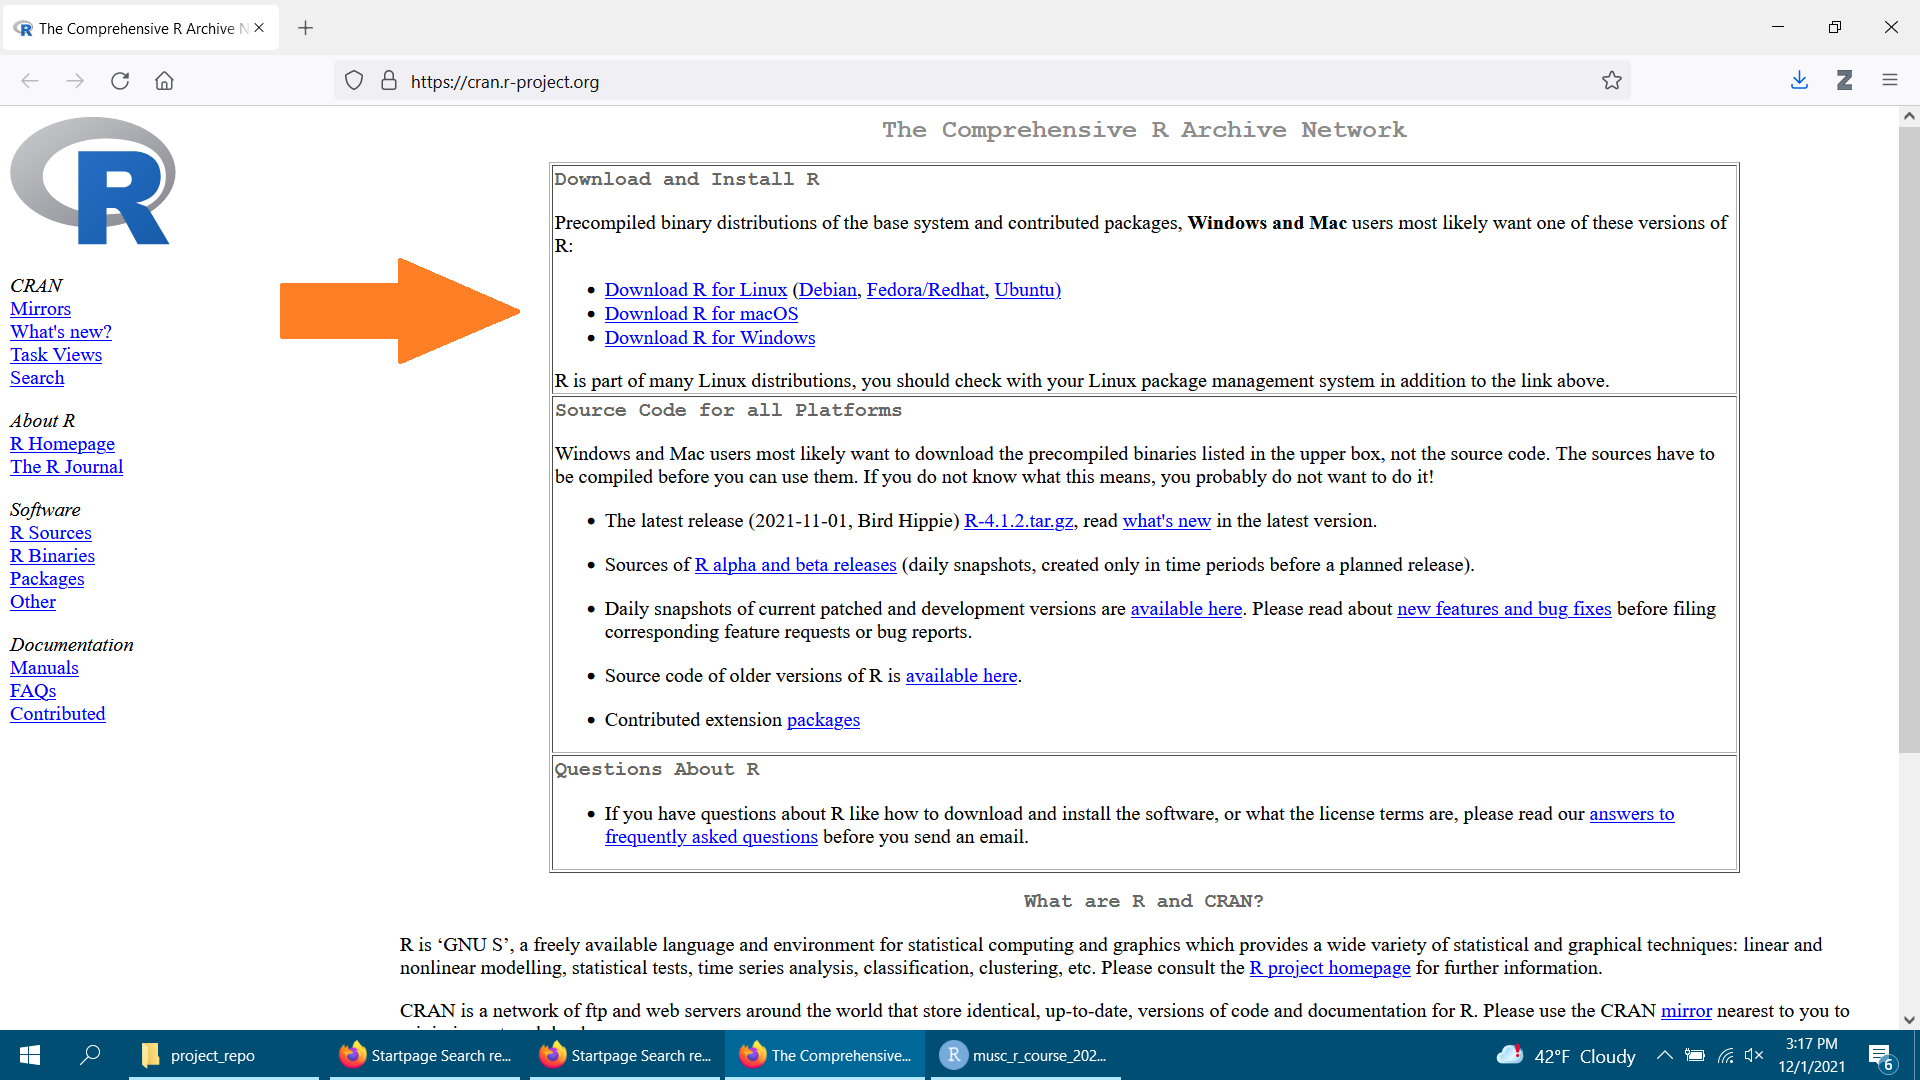
\includegraphics[width=0.8\linewidth]{images/cran_download_instruction} 

}

\caption{https://cran.r-project.org/}\label{fig:unnamed-chunk-2}
\end{figure}

\hypertarget{step-2---download-and-install-the-rstudio-ide}{%
\subsection{Step 2 - Download and install the RStudio IDE}\label{step-2---download-and-install-the-rstudio-ide}}

Several years ago, writing code in R was especially difficult because there was so much to keep track of and it was all hidden behind the code. The RStudio IDE fixed that for us by allowing us to continue coding in R, but this time with a collection of useful windows that keep track of what's happening in our code (e.g., what datasets do we have loaded? what plots have we generated?).

\textbf{After you installed R}, installing the RStudio IDE should be fairly straightforward. Just go to their Downloads page (\href{https://www.rstudio.com/products/rstudio/download/}{\texttt{https://www.rstudio.com/products/rstudio/download/}}) and choose the \textbf{Desktop Version}

\begin{figure}

{\centering 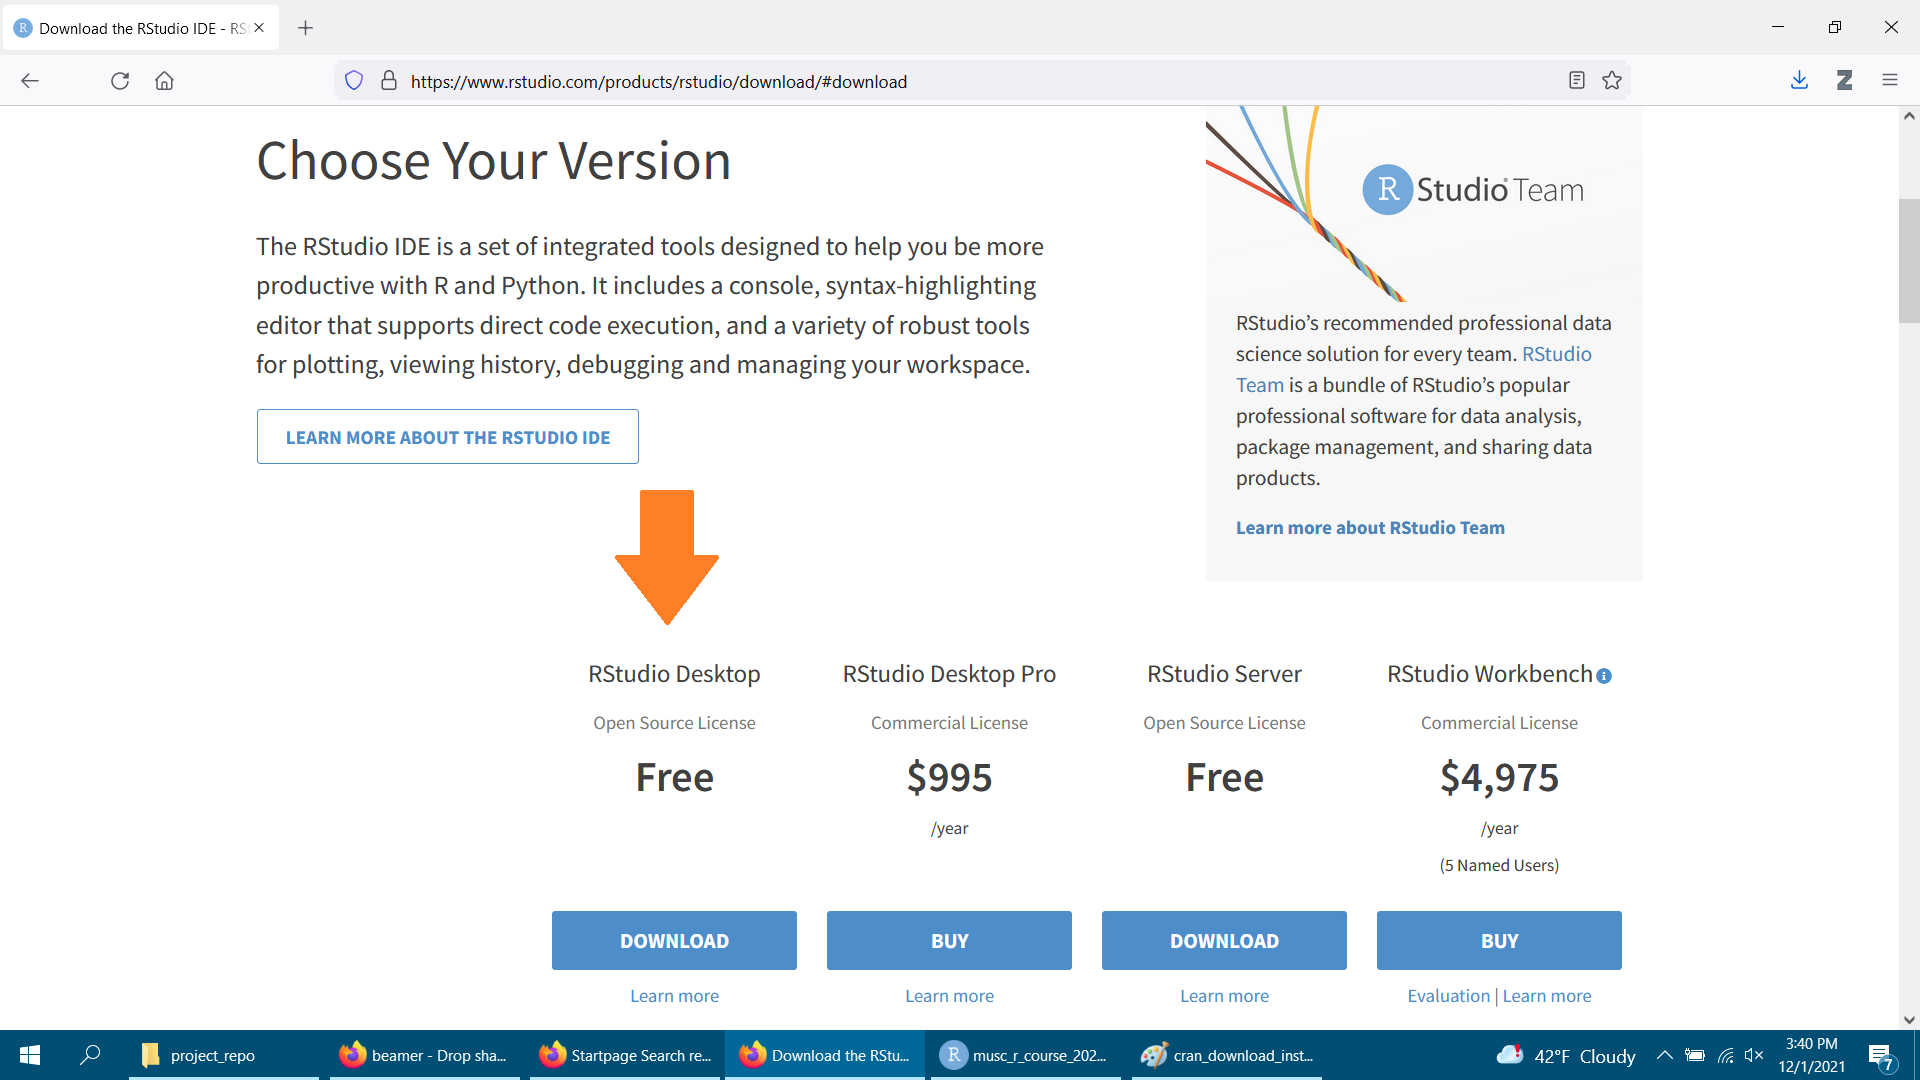
\includegraphics[width=0.8\linewidth]{images/rstudio_download_instruction} 

}

\caption{https://www.rstudio.com/products/rstudio/download/}\label{fig:unnamed-chunk-3}
\end{figure}

\textbf{NOTE:} make sure you finish step 1 first! This will allow you to save several steps linking R and RStudio. This is because if R is installed first, RStudio will do the linking for you automatically.

\hypertarget{step-3---install-the-tidyverse-package-optional}{%
\subsection{\texorpdfstring{Step 3 - Install the \texttt{tidyverse} package (optional)}{Step 3 - Install the tidyverse package (optional)}}\label{step-3---install-the-tidyverse-package-optional}}

Now that both R and RStudio are installed, let's open RStudio and install some packages.

\begin{enumerate}
\def\labelenumi{\arabic{enumi}.}
\item
  Once you have Rstudio open, you should see several windows. Find the Console window.
\item
  Inside that window, type \texttt{install.packages(\textquotesingle{}tidyverse\textquotesingle{})} and press ENTER.

  \begin{itemize}
  \tightlist
  \item
    R is case-sensitive, so make sure to type (or copy/paste) the command exactly.
  \item
    This should start an installation process that takes a few minutes (no more than 10) and will install a package you will use basically every time you program in R - so it's very useful to have.
  \item
    If you get an error message while installing, don't worry! That's pretty common and you've probably still done everything right. Just remind me in class and we will make sure to troubleshoot it for you.
  \end{itemize}
\end{enumerate}

\begin{figure}

{\centering 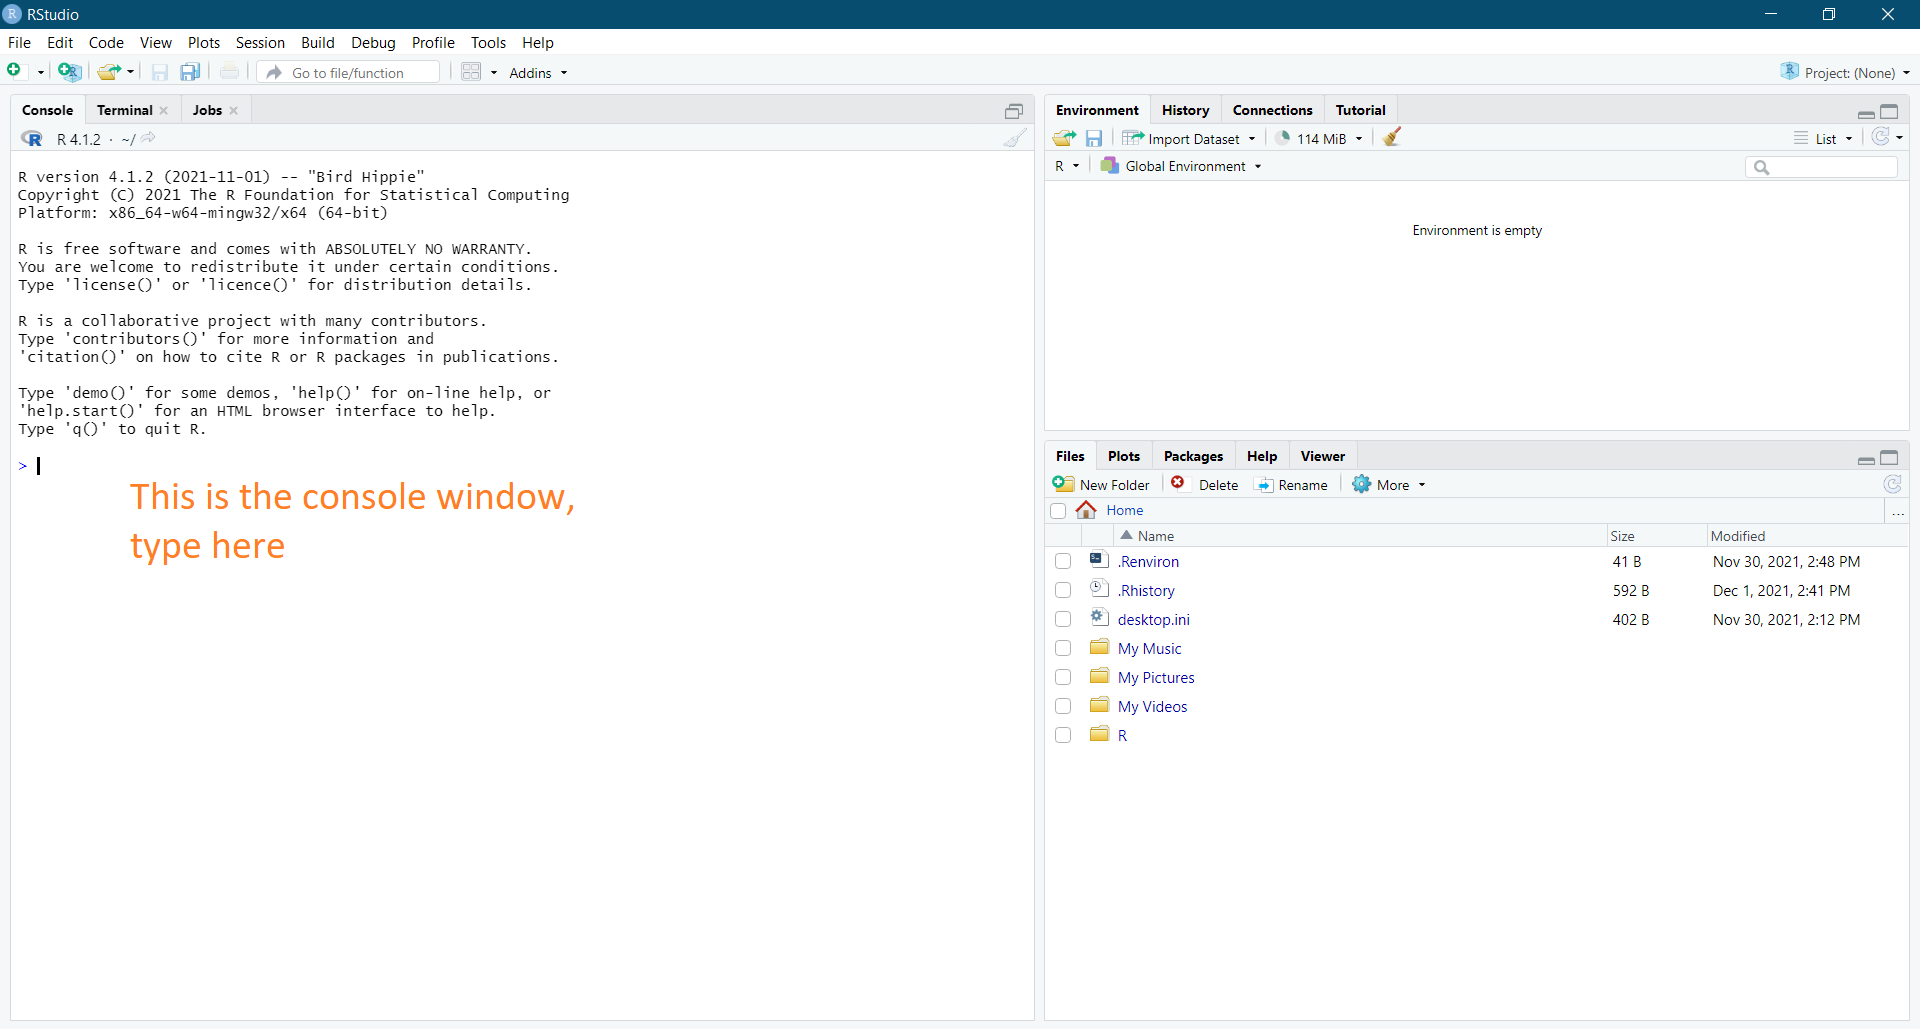
\includegraphics[width=0.8\linewidth]{images/package_install_instructions} 

}

\caption{The RStudio IDE}\label{fig:unnamed-chunk-4}
\end{figure}

\hypertarget{a-tour-of-rstudio}{%
\section{A tour of RStudio}\label{a-tour-of-rstudio}}

If R is a language, RStudio is a chat program that makes it easier to talk to your computer using that language. It includes multiple windows that help you keep track of the different parts of the conversation.

Although there are lots of tabs scattered throughout the overal RStudio application, there are generally 3 that we will use every day.

\hypertarget{the-console}{%
\subsection{The console}\label{the-console}}

Shown in the left half (or sometimes lower left quarter) of the screen. The console is where you can talk to R live. Everything you enter into the console happens right away, which makes it really useful for quick calculations.

\hypertarget{the-environment}{%
\subsection{The environment}\label{the-environment}}

The Environment tab in the top right quadrant shows you every object you currently have imported into R. This is especially useful for keeping track of what you named your datasets (and whether your datasets even made it into R in the first place).

\hypertarget{the-lower-right-pane}{%
\subsection{The lower right pane}\label{the-lower-right-pane}}

There are many tabs in the lower right pane and you'll use most of them on a daily basis. The files tab shows you all the files in your current working directory (the file that R is paying attention to right now). The plots pane shows your plots, assuming you haven't told R to send them somewhere else. Lastly, the help pane will show you R's (very useful) help documentation, anytime you put a \texttt{?} in front of a command (e.g., \texttt{?lm()} brings up the help file for the \texttt{lm()} command).

\begin{figure}

{\centering 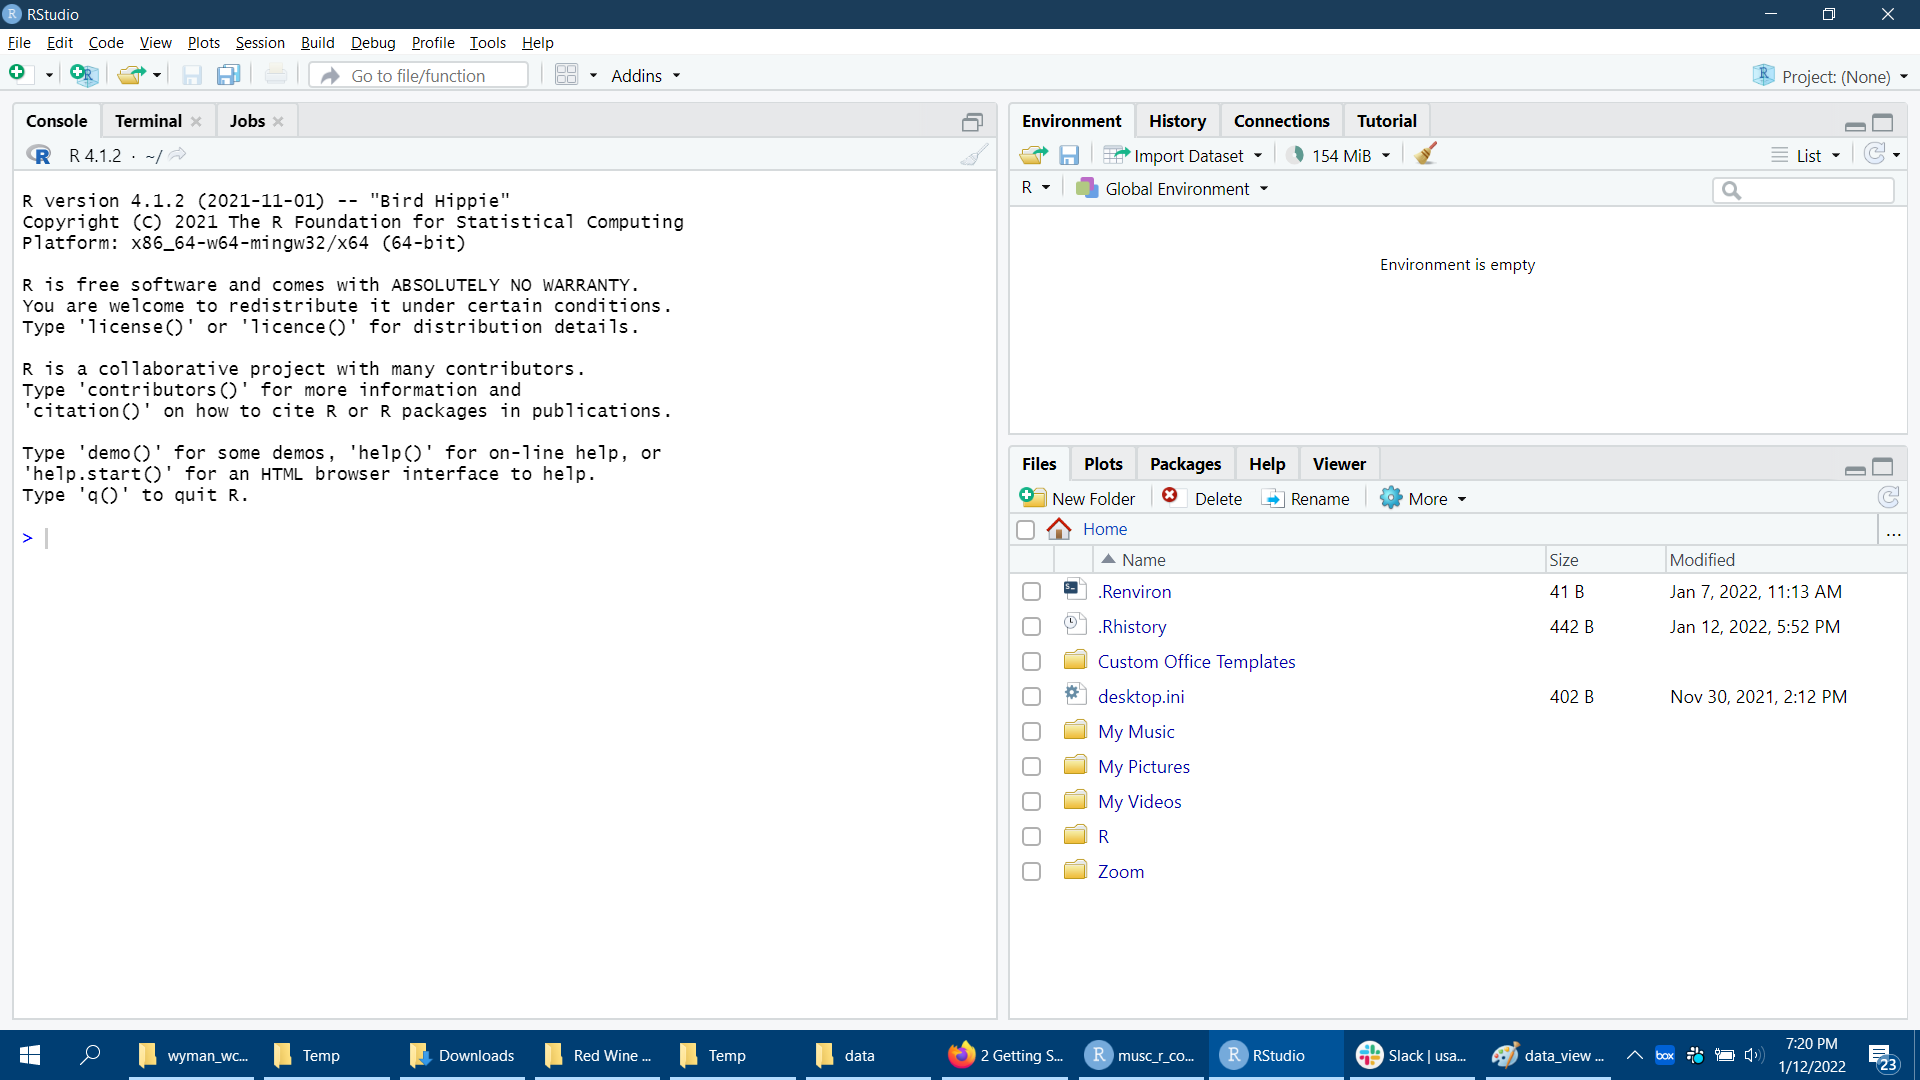
\includegraphics[width=0.8\linewidth]{images/rstudio} 

}

\caption{The RStudio IDE}\label{fig:unnamed-chunk-5}
\end{figure}

\hypertarget{your-very-first-analysis}{%
\section{Your very first analysis}\label{your-very-first-analysis}}

To give us a roadmap for our future work in R, we'll start with a basic analysis here. For demonstration purposes, we'll be doing a basic analysis of red wine and checking whether its chemical properties predict how well it's rated by professional tasters.

\hypertarget{step-1---download-the-data}{%
\subsection{Step 1 - download the data}\label{step-1---download-the-data}}

The first step is simply to download the data, \textbf{\href{https://www.kaggle.com/uciml/red-wine-quality-cortez-et-al-2009/download}{which can be downloaded here}.}

You might be asked to create a Kaggle account or to log in with Google. Don't worry though, it's totally free.

\hypertarget{step-2---make-an-rstudio-project}{%
\subsection{Step 2 - Make an RStudio Project}\label{step-2---make-an-rstudio-project}}

Now that we have our data, we need a place to store it - along with all the other important things we'll be working on, like our code and analysis output. The best option is to create an RStudio Project, which is a special kind of folder that RStudio knows to keep track of. RStudio projects have a number of advantages, but for now all you need to know is that they make it easier to keep track of your data.

To make a project\ldots{}

\begin{enumerate}
\def\labelenumi{\arabic{enumi}.}
\tightlist
\item
  Navigate to File \textgreater\textgreater{} New Project (sometimes this takes a few seconds to load after you click on it)
\item
  Select New Directory
\item
  Select New Project
\item
  In the Directory Name text box, write the name for your project. In this case, a good name might be something like ``Red Wine Practice''.

  \begin{itemize}
  \tightlist
  \item
    Note, you can change the directory you want your project folder too, but it's not necessary for this example.
  \item
    Leave all the remaining boxes (Create git repository, Use renv with this project) \textbf{unchecked}.
  \end{itemize}
\item
  Click Create Project
\end{enumerate}

With your project now created, you should now see ``Red Wine Practice'' (or whatever you named your project in the top of your RStudio application window). Moreover, if you look to the Files pane on the lower right, you should see a file called \texttt{Red\ Wine\ Practice.Rproj}. Lastly, you should notice that your working directory is now called ``Red Wine Practice''.

You can double-check this by typing \texttt{getwd()} (short for ``get working directory'') into the R Console on the bottom left and hit ENTER.

\hypertarget{step-3---get-the-data-into-your-project-folder}{%
\subsection{Step 3 - Get the data into your project folder}\label{step-3---get-the-data-into-your-project-folder}}

The quickest way to get your data into your project folder, is simply to copy/paste the \texttt{winequality-red.csv} you downloaded in Step 1 into your Red Wine Practice folder.

Where is that practice folder? Again, you can get the full path for your project folder simply by typing \texttt{getwd()} into the R console on the lower left and hitting ENTER.

To check whether your copy/paste operation worked, your can type \texttt{list.files()} into the R console. If it worked, you should see it listed along with your \texttt{Red\ Wine\ Practice.Rproj}

\begin{figure}

{\centering 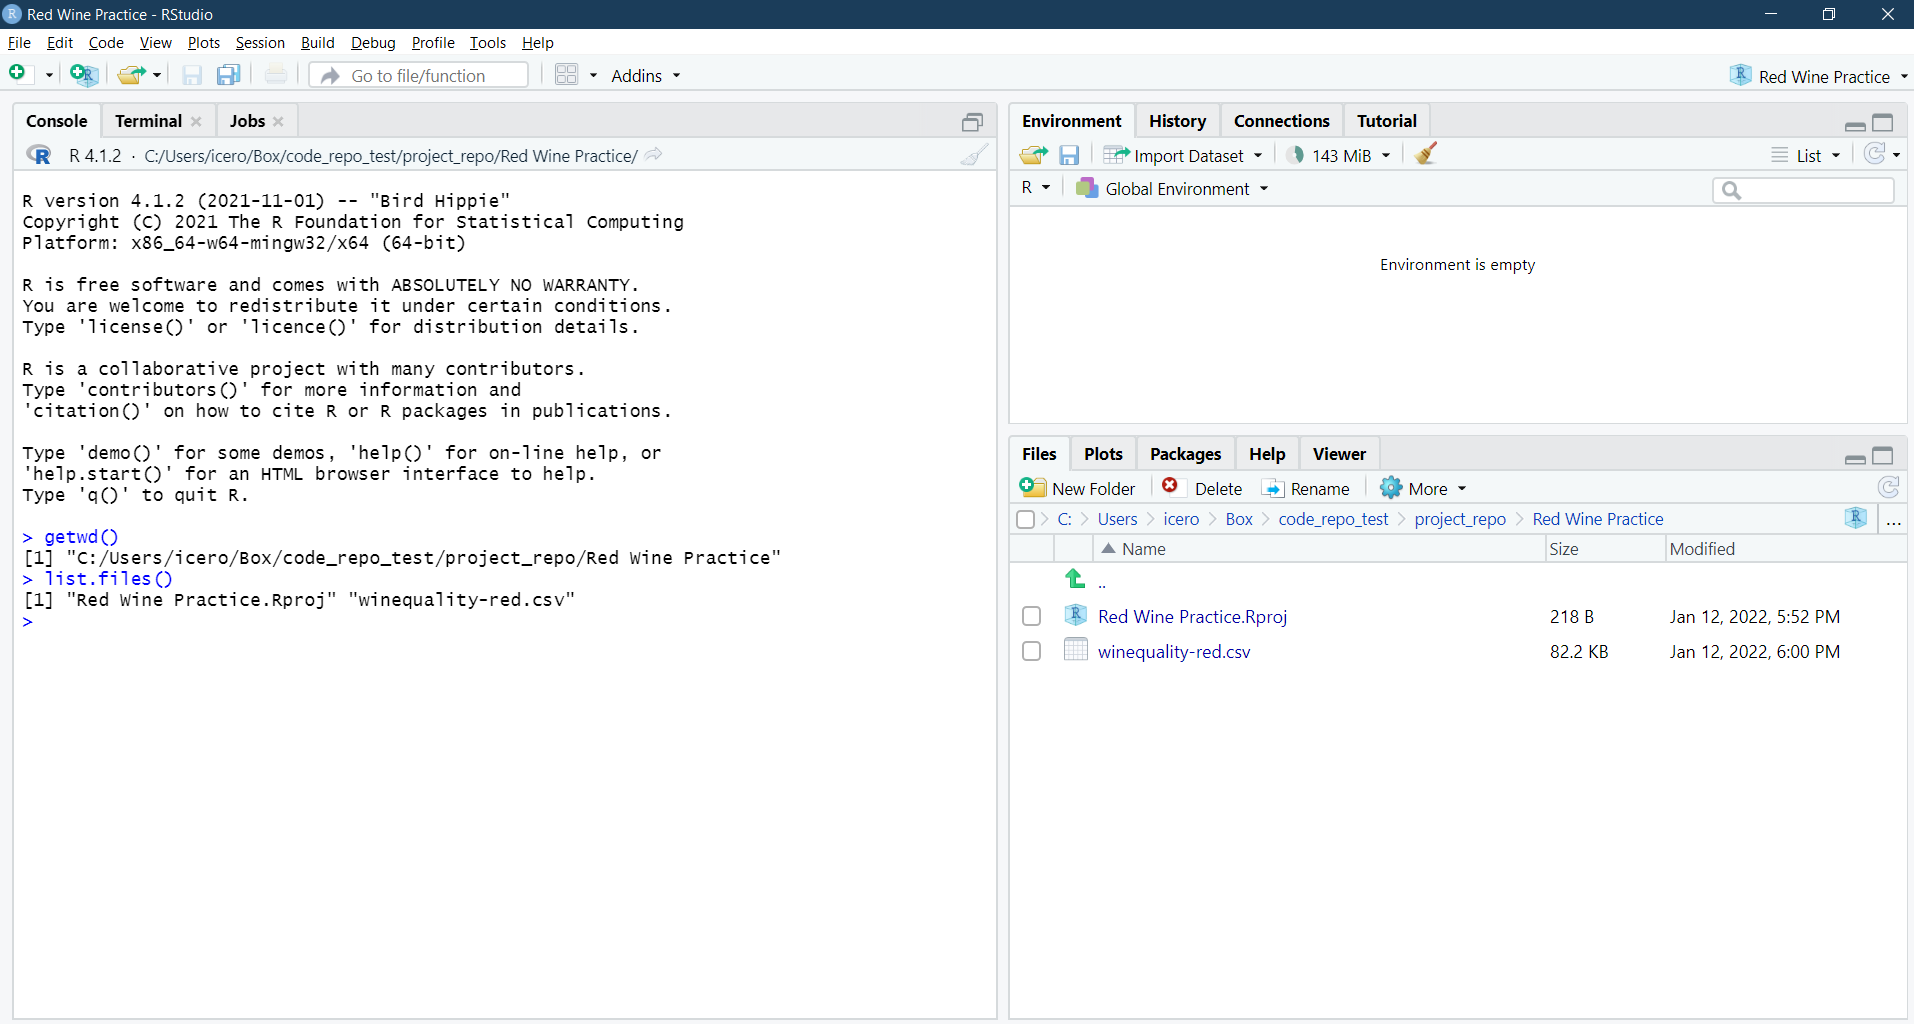
\includegraphics[width=1\linewidth]{images/rproj_data_import} 

}

\caption{Checking the copy/paste operation worked with `list.files()`}\label{fig:unnamed-chunk-6}
\end{figure}

\hypertarget{step-4---open-an-rmarkdown-notebook}{%
\subsection{Step 4 - Open an Rmarkdown Notebook}\label{step-4---open-an-rmarkdown-notebook}}

We need a place to type our R commands, plus some notes to ourselves. The best way to do both of those things at the same time as an Rmarkdown notebook.

\begin{enumerate}
\def\labelenumi{\arabic{enumi}.}
\tightlist
\item
  Navigate to File \textgreater\textgreater{} New file \textgreater\textgreater{} R Notebook

  \begin{itemize}
  \tightlist
  \item
    \textbf{NOTE}: You might get a message asking if you want to install some packages. Press OK / Yes - you \emph{do} want to install them.
  \end{itemize}
\item
  With the new notebook file opened, press CTRL+S to save the file under a different name. You can use whatever name you want. For this example, I will use \texttt{main.Rmd} to remind myself this is my main analysis file.
\item
  Inside your newly saved file, change the title from ``R Notebook'' to something more descriptive like ``My first wine analysis''.
\item
  Lastly, RStudio gave us a bunch of boilerplate code. We won't need that today, so delete everything below the second \texttt{-\/-\/-} at the top of the page, right under \texttt{output:\ html\_notebook}. Your final document should then look something like the following.
\end{enumerate}

\begin{figure}

{\centering 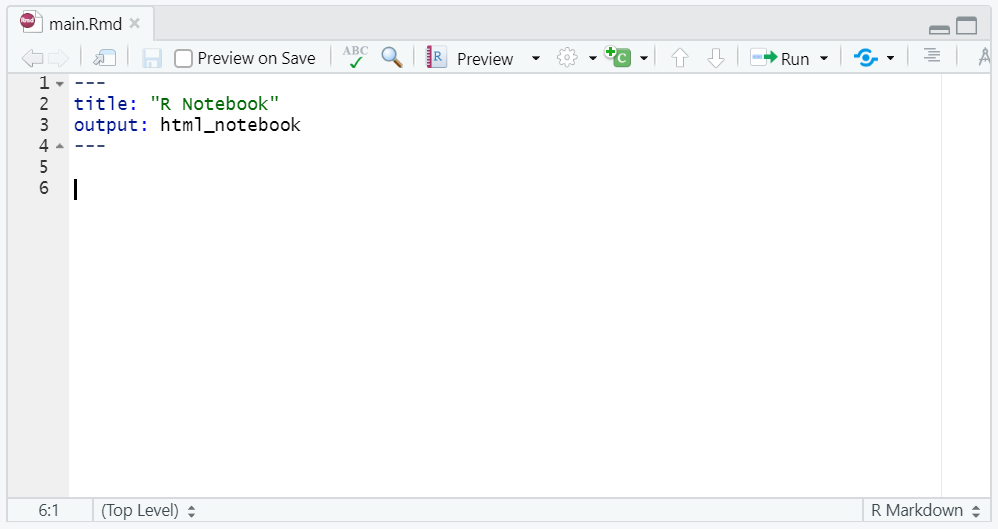
\includegraphics[width=0.8\linewidth]{images/rmarkdown_setup} 

}

\caption{What your Rmarkdown file should look like before we start coding}\label{fig:unnamed-chunk-7}
\end{figure}

\hypertarget{step-5---create-a-space-to-code}{%
\subsection{Step 5 - Create a space to code}\label{step-5---create-a-space-to-code}}

Rmarkdown documents have whitespace and greyspace. Whitespace is where you type notes to yourself. Greyspace is where you type R commands. We call these greyspaces \textbf{code blocks}.

\begin{enumerate}
\def\labelenumi{\arabic{enumi}.}
\tightlist
\item
  Anywhere below line 4, type a note to yourself like ``This is where I imported the data.''
\item
  Move your curser to a line below that note you just wrote (e.g., line 8). Then, press CTRL+ALT+I. This will create a grey codeblock.
\end{enumerate}

\begin{figure}

{\centering 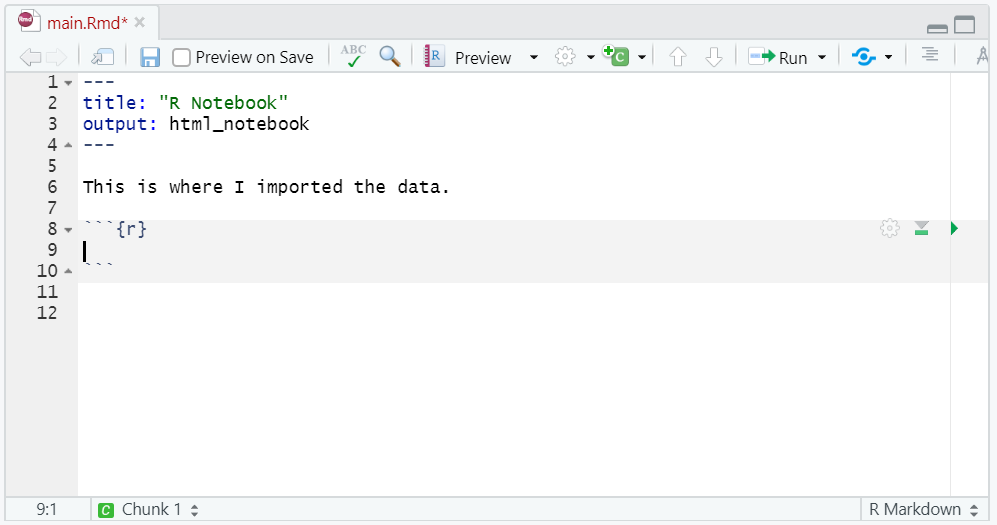
\includegraphics[width=0.8\linewidth]{images/code_block} 

}

\caption{Adding a note to yourself and a grey code block}\label{fig:unnamed-chunk-8}
\end{figure}

\hypertarget{step-6---write-a-command-to-import-the-data}{%
\subsection{Step 6 - Write a command to import the data}\label{step-6---write-a-command-to-import-the-data}}

Importing data involves four things: the name of the datafile, a command to read the data into R, the ``assignment operator'' (written as \texttt{\textless{}-}), and the name you want R to call the imported data when you reference it later. Fortunately, this \emph{sounds} much more complicated than it is.

For now, just copy and paste the following commmand into the middle of your grey code block (for me, that is line 9).

\begin{Shaded}
\begin{Highlighting}[]
\NormalTok{my\_data }\OtherTok{\textless{}{-}} \FunctionTok{read.csv}\NormalTok{(}\StringTok{\textquotesingle{}winequality{-}red.csv\textquotesingle{}}\NormalTok{)}
\end{Highlighting}
\end{Shaded}

This is R code. It can be translated into English, but it's a little clunky. Also, generally code works from right to left. So, you would read this sentence as something like ``Take the file called \texttt{winequality-red.csv}, read it into R, then call whatever comes out of that process \texttt{my\_data}.''

To get the R code to run, put your cursor inside the grey code block and press CTRL+SHIFT+ENTER. This runs all the code inside that block.

\hypertarget{step-7---look-inside-the-data}{%
\subsection{Step 7 - Look inside the data}\label{step-7---look-inside-the-data}}

Make a new code block a few lines down from the last one. Then type just the name of your imported data and run the block. You should see a preview of your dataset. To scroll through the other variables in the dataset, press the right-facing triangle on the right side of the preview.

\begin{figure}

{\centering 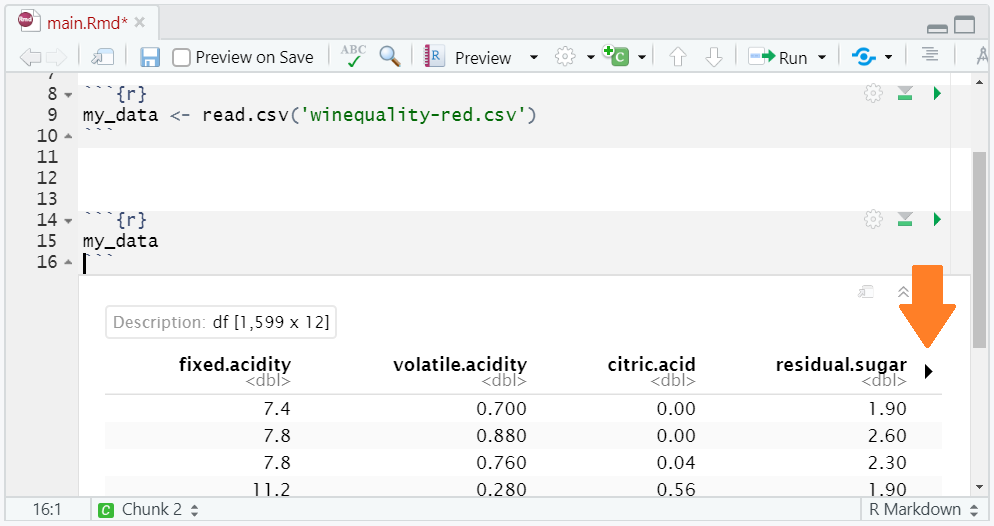
\includegraphics[width=0.8\linewidth]{images/data_view} 

}

\caption{Preview of the data}\label{fig:unnamed-chunk-11}
\end{figure}

\hypertarget{step-8---make-a-histogram}{%
\subsection{Step 8 - Make a histogram}\label{step-8---make-a-histogram}}

I think I'm most interested in the final variable in the dataset, \texttt{quality}. In this case, that is the quality of the wine - rated by professionals on a scale of 1 to 10. Let's see what the distribution looks like. For that we can use the \texttt{hist()} command (short for ``histogram'').

But what should we give our \texttt{hist()} command? We unfortunately can't give it the whole dataset. After all, we only want a histogram of one variable. How do we specify that variable? We use the ``selection operator'', which we write as a \texttt{\$}-symbol, like below.

\begin{Shaded}
\begin{Highlighting}[]
\FunctionTok{hist}\NormalTok{(my\_data}\SpecialCharTok{$}\NormalTok{quality)}
\end{Highlighting}
\end{Shaded}

\begin{figure}

{\centering 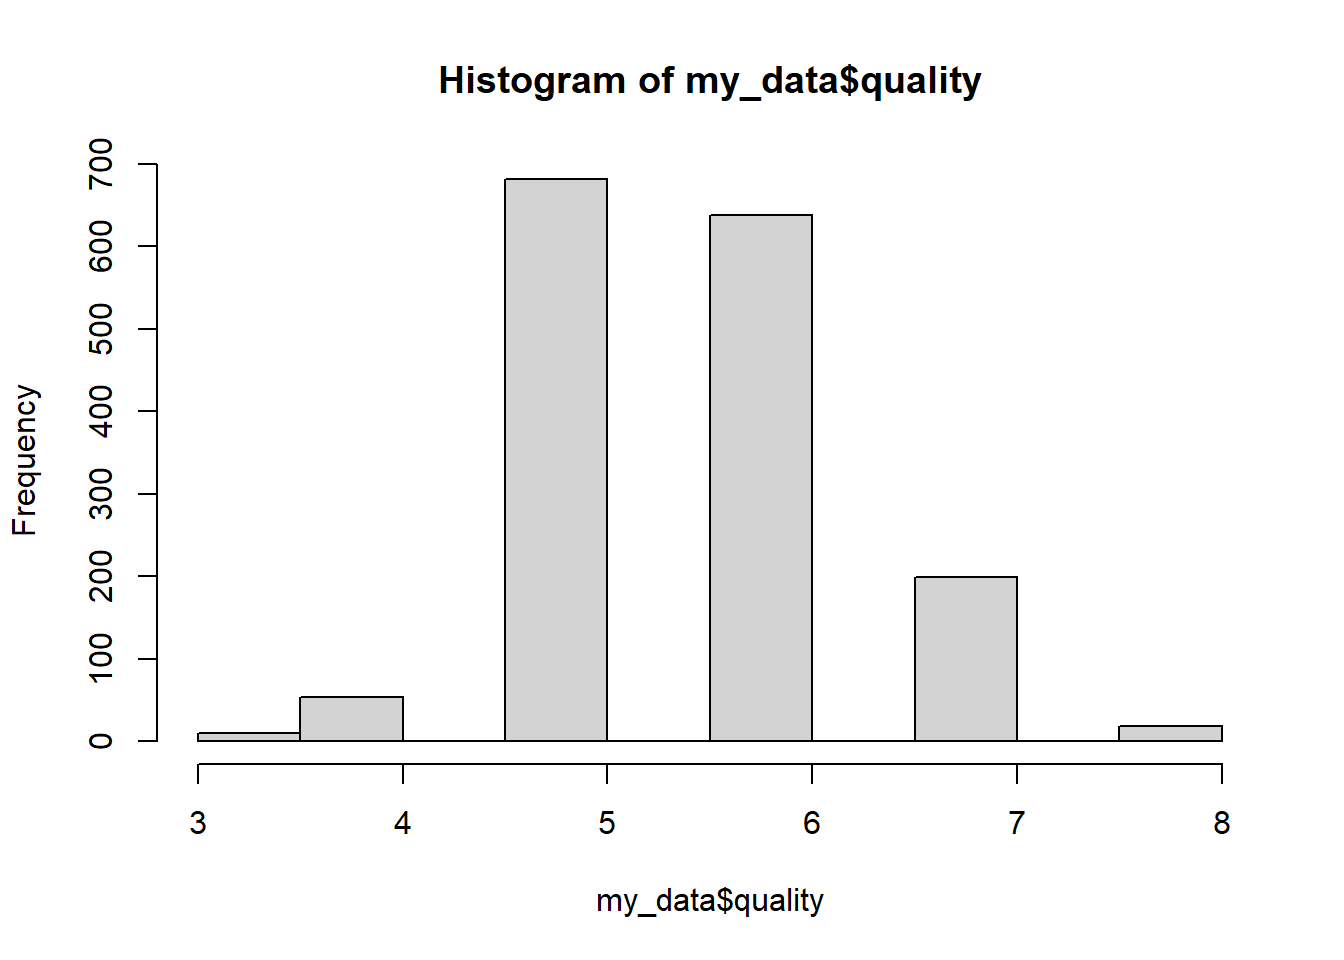
\includegraphics[width=0.8\linewidth]{_main_files/figure-latex/unnamed-chunk-12-1} 

}

\caption{Histogram of wine quality ratings}\label{fig:unnamed-chunk-12}
\end{figure}

\hypertarget{step-9---run-a-regression}{%
\subsection{Step 9 - Run a regression}\label{step-9---run-a-regression}}

Now that we have a sense of what our outcome variable (\texttt{quality}) looks like, let's see if we can investigate some of the chemical characteristics in wine associated with that outcome.

The ones that stick out to me are \texttt{pH} (acidity) and \texttt{alcohol} content because they seem like things that would really affect the taste. Let's use those as our predictors

To run a regression, we need just a few things (out of order):
- The \texttt{lm()} command, which is short for ``linear model''. This is how R will know we want a regression.
- Our data, named \texttt{my\_data}
- A regression formula, which tells R what the outcome variable and it's predictors are
- The assignment operator again (\texttt{\textless{}-}), which tells us where to store the results
- A name for where to store the results

Putting all of that together looks like this. One you have it all typed in (or copy/pasted), run the whole block with CTRL+SHIFT+ENTER.

\begin{Shaded}
\begin{Highlighting}[]
\NormalTok{my\_results }\OtherTok{\textless{}{-}} \FunctionTok{lm}\NormalTok{(}
  \AttributeTok{formula =}\NormalTok{ quality }\SpecialCharTok{\textasciitilde{}}\NormalTok{ pH }\SpecialCharTok{+}\NormalTok{ alcohol,}
  \AttributeTok{data =}\NormalTok{ my\_data)}
\end{Highlighting}
\end{Shaded}

\hypertarget{step-10---get-a-summary-of-your-results}{%
\subsection{Step 10 - Get a summary of your results}\label{step-10---get-a-summary-of-your-results}}

You may have noticed that in Step 9, your results didn't show up anywhere after you ran your regression. That's because R stored them in \texttt{my\_results}, just like it stored the outcome of the \texttt{read.csv()} command in \texttt{my\_data}.

This often surprises people who come from other software packages, but that's okay. Our results are still easy to get. We just need to ask R for a summary of them.

\begin{Shaded}
\begin{Highlighting}[]
\FunctionTok{summary}\NormalTok{(my\_results)}
\end{Highlighting}
\end{Shaded}

\begin{verbatim}
## 
## Call:
## lm(formula = quality ~ pH + alcohol, data = my_data)
## 
## Residuals:
##     Min      1Q  Median      3Q     Max 
## -2.7153 -0.4066 -0.1105  0.5076  2.4584 
## 
## Coefficients:
##             Estimate Std. Error t value Pr(>|t|)    
## (Intercept)  4.42581    0.38742  11.424  < 2e-16 ***
## pH          -0.85011    0.11571  -7.347 3.23e-13 ***
## alcohol      0.38617    0.01676  23.036  < 2e-16 ***
## ---
## Signif. codes:  
## 0 '***' 0.001 '**' 0.01 '*' 0.05 '.' 0.1 ' ' 1
## 
## Residual standard error: 0.6989 on 1596 degrees of freedom
## Multiple R-squared:  0.252,  Adjusted R-squared:  0.2511 
## F-statistic: 268.9 on 2 and 1596 DF,  p-value: < 2.2e-16
\end{verbatim}

This gives us a basic regression table with all of the same information you are used to. Under the \emph{Coefficients} heading, we see the b-values / slopes (Estimate column), their standard errors, t-values, and p-values.

Next to the p-values, we see stars reminding us that our p-values are significant at the \textless{} .001 level. In fact, our p-values are so small, they have to be shown in scientific notation (``3.23e-13''). These can be treated as basically zero.

Lastly, at the very bottom, we also see the usual R-squared values (here, .252), our F-statistic, and degrees of freedom - everything we need to create a publication-ready regression table.

\hypertarget{a-look-forward}{%
\subsection{A Look forward}\label{a-look-forward}}

Over the last 10 steps, we ran through a basic version of essentially every R analysis you are likely to conduct in the future. This is example thus contains a useful workflow you will likely want to recreate in your future work:

\begin{itemize}
\tightlist
\item
  Create a project to store everything
\item
  Import the data
\item
  Visualize / explore the data
\item
  Run main analysis model
\item
  Summarize results
\end{itemize}

Although the data and models you use might be more complicated as your time in R progresses, it's helpful to remember that everything your are doing typically reduces to these fundamental steps.

\hypertarget{basic-r}{%
\chapter{Basic R}\label{basic-r}}

\hypertarget{writing-in-r-and-rmarkdown}{%
\section{Writing in R and Rmarkdown}\label{writing-in-r-and-rmarkdown}}

\hypertarget{chatting-with-r}{%
\subsection{Chatting with R}\label{chatting-with-r}}

Using R is just a chat with the computer.

``Hey, R. What is \(1 + 2\)?''

\begin{Shaded}
\begin{Highlighting}[]
\DecValTok{1} \SpecialCharTok{+} \DecValTok{2}
\end{Highlighting}
\end{Shaded}

\begin{verbatim}
## [1] 3
\end{verbatim}

\hypertarget{rmarkdown-tricks}{%
\subsection{Rmarkdown tricks}\label{rmarkdown-tricks}}

\begin{itemize}
\tightlist
\item
  To make text \textbf{bold}, we add two **s around it.
\item
  To make text \emph{italicized}, we add just one * around it.
\item
  If we need special characters (like * or \$), then we just add a forward ``\textbackslash{}'' in front of them (but not behind).
\item
  Math symbols in your text are process with Latex, just put an ``\$'' before and after your math. Like this, \$y = x\$ becomes \(y = x\).
\end{itemize}

\hypertarget{code-blocks}{%
\subsection{Code blocks}\label{code-blocks}}

To make a code block, press CTRL+ALT+I.

\begin{Shaded}
\begin{Highlighting}[]
\NormalTok{banana }\OtherTok{\textless{}{-}} \DecValTok{5}
\NormalTok{banana }\SpecialCharTok{+} \DecValTok{1}
\end{Highlighting}
\end{Shaded}

\begin{verbatim}
## [1] 6
\end{verbatim}

\hypertarget{variables}{%
\section{Variables}\label{variables}}

Variables are values that I want to give names to and save for later.

\hypertarget{the-assignment-operator}{%
\subsection{The assignment operator}\label{the-assignment-operator}}

We make variables with the \texttt{\textless{}-} operator. This is called the \emph{assignment operator} because it assigns values on the right to names on the left. If I want to know what the value of a variable is, I can run it alone on its own line.

\begin{Shaded}
\begin{Highlighting}[]
\NormalTok{my\_special\_var }\OtherTok{\textless{}{-}} \DecValTok{1} \SpecialCharTok{+} \DecValTok{2}
\NormalTok{my\_special\_var}
\end{Highlighting}
\end{Shaded}

\begin{verbatim}
## [1] 3
\end{verbatim}

You can TECHNICALLY use \texttt{=} for assignment too. Never do this.

\begin{Shaded}
\begin{Highlighting}[]
\NormalTok{my\_other\_var }\OtherTok{=} \DecValTok{12}
\NormalTok{my\_other\_var }\SpecialCharTok{+}\NormalTok{ my\_special\_var}
\end{Highlighting}
\end{Shaded}

\begin{verbatim}
## [1] 15
\end{verbatim}

The \texttt{=} symbol gets also used for a few other things in R. So, using it to assign variables will make your code more confusing to you, when you go back to read it over later.

\hypertarget{numerics}{%
\subsection{Numerics}\label{numerics}}

\textbf{Doubles}

Doubles are decimal numbers, like \(1.1, 2.2, 3.0\). If I make a number variable without doing anything special, R defaults to a double.

\begin{Shaded}
\begin{Highlighting}[]
\NormalTok{a }\OtherTok{\textless{}{-}} \FloatTok{1.1}
\NormalTok{b }\OtherTok{\textless{}{-}} \FloatTok{2.0}
\FunctionTok{is.double}\NormalTok{(a)}
\end{Highlighting}
\end{Shaded}

\begin{verbatim}
## [1] TRUE
\end{verbatim}

\begin{Shaded}
\begin{Highlighting}[]
\FunctionTok{is.double}\NormalTok{(b)}
\end{Highlighting}
\end{Shaded}

\begin{verbatim}
## [1] TRUE
\end{verbatim}

\textbf{Integers}

Integers must have an \texttt{L} after them. That is how R knows that you don't want a double, but instead want a ``long-capable integer''.

\begin{Shaded}
\begin{Highlighting}[]
\NormalTok{c }\OtherTok{\textless{}{-}}\NormalTok{ 1L}
\NormalTok{d }\OtherTok{\textless{}{-}} \DecValTok{1}
\FunctionTok{is.integer}\NormalTok{(c)}
\end{Highlighting}
\end{Shaded}

\begin{verbatim}
## [1] TRUE
\end{verbatim}

\begin{Shaded}
\begin{Highlighting}[]
\FunctionTok{is.integer}\NormalTok{(d)}
\end{Highlighting}
\end{Shaded}

\begin{verbatim}
## [1] FALSE
\end{verbatim}

Here is a useful cheatsheet for the different numeric operators and how they behave.

\begin{tabular}{c|c|c}
\hline
Operator & Expression & Result\\
\hline
+ & 10 + 3 & 13\\
\hline
- & 10 - 3 & 7\\
\hline
* & 10 * 3 & 30\\
\hline
/ & 10 / 3 & 3.333\\
\hline
\textasciicircum{} & 10 \textasciicircum{} 3 & 1000\\
\hline
\%/\% & 10 \%/\% 3 & 3\\
\hline
\%\% & 10 \%\% 3 & 1\\
\hline
\end{tabular}

\textbf{Why care about the difference?}

Almost 99\% of the time, this wont matter. But, with big data, integers take up must less memory.

\begin{Shaded}
\begin{Highlighting}[]
\NormalTok{my\_integers }\OtherTok{\textless{}{-}} \FunctionTok{seq}\NormalTok{(}\AttributeTok{from =}\NormalTok{ 1L, }\AttributeTok{to =} \FloatTok{1e6}\NormalTok{L, }\AttributeTok{by =}\NormalTok{ 1L)}
\NormalTok{my\_doubles }\OtherTok{\textless{}{-}} \FunctionTok{seq}\NormalTok{(}\AttributeTok{from =} \FloatTok{1.0}\NormalTok{, }\AttributeTok{to =} \FloatTok{1e6}\NormalTok{, }\AttributeTok{by =} \FloatTok{1.0}\NormalTok{)}
\FunctionTok{object.size}\NormalTok{(my\_integers)}
\end{Highlighting}
\end{Shaded}

\begin{verbatim}
## 4000048 bytes
\end{verbatim}

\begin{Shaded}
\begin{Highlighting}[]
\FunctionTok{object.size}\NormalTok{(my\_doubles)}
\end{Highlighting}
\end{Shaded}

\begin{verbatim}
## 8000048 bytes
\end{verbatim}

Note here that although we are using only whole numbers from 1 to 1 million, the first sequence (\texttt{my\_integers}) is stored as an integer and the second sequence (\texttt{my\_doubles}) is stored as a number that may include decimals. This second case needs more space (twice as much) to be allocated in advance, even if we never use those decimal places.

Again, this will almost never matter for most people, most of the time. However, it is good to be aware of for when your datasets get large (i.e., several million cases or more).

\hypertarget{characters}{%
\subsection{Characters}\label{characters}}

Characters are text symbols and they are made with either "" or '', either works.

\begin{Shaded}
\begin{Highlighting}[]
\NormalTok{a }\OtherTok{\textless{}{-}} \StringTok{\textquotesingle{}here is someone}\SpecialCharTok{\textbackslash{}\textquotesingle{}}\StringTok{s text\textquotesingle{}}
\NormalTok{b }\OtherTok{\textless{}{-}} \StringTok{"here is more text"}
\NormalTok{a}
\end{Highlighting}
\end{Shaded}

\begin{verbatim}
## [1] "here is someone's text"
\end{verbatim}

\begin{Shaded}
\begin{Highlighting}[]
\NormalTok{b}
\end{Highlighting}
\end{Shaded}

\begin{verbatim}
## [1] "here is more text"
\end{verbatim}

To combine two strings, I use \texttt{paste()}.

\begin{Shaded}
\begin{Highlighting}[]
\FunctionTok{paste}\NormalTok{(a, b)}
\end{Highlighting}
\end{Shaded}

\begin{verbatim}
## [1] "here is someone's text here is more text"
\end{verbatim}

If I dont want a space, then I used \texttt{paste0()}.

\begin{Shaded}
\begin{Highlighting}[]
\FunctionTok{paste0}\NormalTok{(a, b)}
\end{Highlighting}
\end{Shaded}

\begin{verbatim}
## [1] "here is someone's texthere is more text"
\end{verbatim}

\hypertarget{booleans}{%
\subsection{Booleans}\label{booleans}}

These are True and False values. You make them with the symbols \texttt{T} or \texttt{TRUE} and \texttt{F} or \texttt{FALSE}.

\begin{Shaded}
\begin{Highlighting}[]
\NormalTok{x }\OtherTok{\textless{}{-}}\NormalTok{ T}
\NormalTok{y }\OtherTok{\textless{}{-}}\NormalTok{ F}
\end{Highlighting}
\end{Shaded}

To compare them, we can use three operators.

\begin{itemize}
\tightlist
\item
  \texttt{\&} is ``and''
\item
  \texttt{\textbar{}} is ``or''
\item
  \texttt{!} is ``not'' (just give me the opposite of whatever is after me)
\end{itemize}

\begin{Shaded}
\begin{Highlighting}[]
\NormalTok{x }\SpecialCharTok{\&}\NormalTok{ y }\CommentTok{\# false}
\end{Highlighting}
\end{Shaded}

\begin{verbatim}
## [1] FALSE
\end{verbatim}

\begin{Shaded}
\begin{Highlighting}[]
\NormalTok{x }\SpecialCharTok{|}\NormalTok{ y }\CommentTok{\# true}
\end{Highlighting}
\end{Shaded}

\begin{verbatim}
## [1] TRUE
\end{verbatim}

\begin{Shaded}
\begin{Highlighting}[]
\NormalTok{x }\SpecialCharTok{\&} \SpecialCharTok{!}\NormalTok{y }\CommentTok{\# true}
\end{Highlighting}
\end{Shaded}

\begin{verbatim}
## [1] TRUE
\end{verbatim}

We can also have nested equations

\begin{Shaded}
\begin{Highlighting}[]
\NormalTok{z }\OtherTok{\textless{}{-}}\NormalTok{ F}
\NormalTok{x }\SpecialCharTok{\&} \SpecialCharTok{!}\NormalTok{(y }\SpecialCharTok{|}\NormalTok{ z) }\CommentTok{\# true}
\end{Highlighting}
\end{Shaded}

\begin{verbatim}
## [1] TRUE
\end{verbatim}

We can also compare numbers.

\begin{Shaded}
\begin{Highlighting}[]
\NormalTok{a }\OtherTok{\textless{}{-}} \DecValTok{1}
\NormalTok{b }\OtherTok{\textless{}{-}} \DecValTok{2}
\end{Highlighting}
\end{Shaded}

\begin{Shaded}
\begin{Highlighting}[]
\NormalTok{a }\SpecialCharTok{\textless{}} \DecValTok{1}
\end{Highlighting}
\end{Shaded}

\begin{verbatim}
## [1] FALSE
\end{verbatim}

\begin{Shaded}
\begin{Highlighting}[]
\NormalTok{a }\SpecialCharTok{\textless{}=} \DecValTok{1}
\end{Highlighting}
\end{Shaded}

\begin{verbatim}
## [1] TRUE
\end{verbatim}

\begin{Shaded}
\begin{Highlighting}[]
\NormalTok{a }\SpecialCharTok{==} \DecValTok{1}
\end{Highlighting}
\end{Shaded}

\begin{verbatim}
## [1] TRUE
\end{verbatim}

If I want to compare multiple numbers, I need to do it seperately.

\begin{Shaded}
\begin{Highlighting}[]
\NormalTok{(a }\SpecialCharTok{\textgreater{}} \DecValTok{1}\NormalTok{) }\SpecialCharTok{|}\NormalTok{ (b }\SpecialCharTok{\textgreater{}} \DecValTok{1}\NormalTok{)}
\end{Highlighting}
\end{Shaded}

\begin{verbatim}
## [1] TRUE
\end{verbatim}

Remember that booleans are ultimately numeric values underneath.

\begin{Shaded}
\begin{Highlighting}[]
\NormalTok{d }\OtherTok{\textless{}{-}}\NormalTok{ T}
\NormalTok{k }\OtherTok{\textless{}{-}}\NormalTok{ F}
\NormalTok{u }\OtherTok{\textless{}{-}} \DecValTok{5}
\NormalTok{d}\SpecialCharTok{*}\NormalTok{u}
\end{Highlighting}
\end{Shaded}

\begin{verbatim}
## [1] 5
\end{verbatim}

\begin{Shaded}
\begin{Highlighting}[]
\NormalTok{d}\SpecialCharTok{*}\NormalTok{k}
\end{Highlighting}
\end{Shaded}

\begin{verbatim}
## [1] 0
\end{verbatim}

\begin{Shaded}
\begin{Highlighting}[]
\FunctionTok{as.numeric}\NormalTok{(d)}
\end{Highlighting}
\end{Shaded}

\begin{verbatim}
## [1] 1
\end{verbatim}

\begin{Shaded}
\begin{Highlighting}[]
\FunctionTok{as.numeric}\NormalTok{(k)}
\end{Highlighting}
\end{Shaded}

\begin{verbatim}
## [1] 0
\end{verbatim}

\hypertarget{special-types}{%
\subsection{Special types}\label{special-types}}

\texttt{NA} - missing

\begin{Shaded}
\begin{Highlighting}[]
\FunctionTok{is.na}\NormalTok{(}\ConstantTok{NA}\NormalTok{)}
\end{Highlighting}
\end{Shaded}

\begin{verbatim}
## [1] TRUE
\end{verbatim}

\texttt{NaN} - you did math wrong

\begin{Shaded}
\begin{Highlighting}[]
\DecValTok{0}\SpecialCharTok{/}\DecValTok{0}
\end{Highlighting}
\end{Shaded}

\begin{verbatim}
## [1] NaN
\end{verbatim}

\texttt{Inf} - infinity

\begin{Shaded}
\begin{Highlighting}[]
\SpecialCharTok{{-}}\DecValTok{5}\SpecialCharTok{/}\DecValTok{0}
\end{Highlighting}
\end{Shaded}

\begin{verbatim}
## [1] -Inf
\end{verbatim}

\hypertarget{vectors}{%
\section{Vectors}\label{vectors}}

R is built is on vectors. Vectors are collections of a bunch of values of the same type.

\begin{Shaded}
\begin{Highlighting}[]
\NormalTok{my\_vec }\OtherTok{\textless{}{-}} \FunctionTok{c}\NormalTok{(}\DecValTok{1}\NormalTok{, }\DecValTok{5}\NormalTok{, }\DecValTok{3}\NormalTok{, }\DecValTok{7}\NormalTok{)}
\NormalTok{my\_vec}
\end{Highlighting}
\end{Shaded}

\begin{verbatim}
## [1] 1 5 3 7
\end{verbatim}

If I try to put different types together, they go to the most primitive type (usually a character string).

\begin{Shaded}
\begin{Highlighting}[]
\NormalTok{my\_other\_vec }\OtherTok{\textless{}{-}} \FunctionTok{c}\NormalTok{(}\DecValTok{22}\NormalTok{, }\StringTok{\textquotesingle{}orange\textquotesingle{}}\NormalTok{, T)}
\NormalTok{my\_other\_vec}
\end{Highlighting}
\end{Shaded}

\begin{verbatim}
## [1] "22"     "orange" "TRUE"
\end{verbatim}

\begin{Shaded}
\begin{Highlighting}[]
\NormalTok{my\_third\_vec }\OtherTok{\textless{}{-}} \FunctionTok{c}\NormalTok{(T, F, }\DecValTok{35}\NormalTok{)}
\NormalTok{my\_third\_vec}
\end{Highlighting}
\end{Shaded}

\begin{verbatim}
## [1]  1  0 35
\end{verbatim}

We can also missing values.

\begin{Shaded}
\begin{Highlighting}[]
\NormalTok{my\_fourth\_vec }\OtherTok{\textless{}{-}} \FunctionTok{c}\NormalTok{(}\DecValTok{1}\NormalTok{, }\DecValTok{4}\NormalTok{, }\DecValTok{5}\NormalTok{, }\ConstantTok{NA}\NormalTok{)}
\NormalTok{my\_fourth\_vec}
\end{Highlighting}
\end{Shaded}

\begin{verbatim}
## [1]  1  4  5 NA
\end{verbatim}

\begin{Shaded}
\begin{Highlighting}[]
\FunctionTok{is.na}\NormalTok{(my\_fourth\_vec)}
\end{Highlighting}
\end{Shaded}

\begin{verbatim}
## [1] FALSE FALSE FALSE  TRUE
\end{verbatim}

If I want to combine two vectors\ldots{}

\begin{Shaded}
\begin{Highlighting}[]
\NormalTok{a }\OtherTok{\textless{}{-}} \FunctionTok{c}\NormalTok{(}\DecValTok{1}\NormalTok{, }\DecValTok{2}\NormalTok{, }\DecValTok{3}\NormalTok{)}
\NormalTok{b }\OtherTok{\textless{}{-}} \FunctionTok{c}\NormalTok{(}\DecValTok{3}\NormalTok{, }\DecValTok{5}\NormalTok{, }\DecValTok{7}\NormalTok{)}
\FunctionTok{c}\NormalTok{(a, b)}
\end{Highlighting}
\end{Shaded}

\begin{verbatim}
## [1] 1 2 3 3 5 7
\end{verbatim}

A brief example of matrices

\begin{Shaded}
\begin{Highlighting}[]
\FunctionTok{matrix}\NormalTok{(}
  \AttributeTok{data =} \FunctionTok{c}\NormalTok{(a, b),}
  \AttributeTok{nrow =} \DecValTok{2}\NormalTok{,}
  \AttributeTok{byrow =}\NormalTok{ T)}
\end{Highlighting}
\end{Shaded}

\begin{verbatim}
##      [,1] [,2] [,3]
## [1,]    1    2    3
## [2,]    3    5    7
\end{verbatim}

Sometimes I want special vectors, direct sequences of numbers. There are two ways to do this. If all I want is a integer sequence (made of doubles), then I use the ``\texttt{\textless{}first\ number\textgreater{}:\textless{}last\ number\textgreater{}}''.

\begin{Shaded}
\begin{Highlighting}[]
\DecValTok{1}\SpecialCharTok{:}\DecValTok{5}
\end{Highlighting}
\end{Shaded}

\begin{verbatim}
## [1] 1 2 3 4 5
\end{verbatim}

\begin{Shaded}
\begin{Highlighting}[]
\DecValTok{5}\SpecialCharTok{:}\DecValTok{1}
\end{Highlighting}
\end{Shaded}

\begin{verbatim}
## [1] 5 4 3 2 1
\end{verbatim}

Other times, I need to count by something other than one, so I use \texttt{seq(from\ =\ \textless{}start\textgreater{},\ to\ =\ \textless{}end\textgreater{},\ by\ =\ \textless{}number\ to\ count\ by\textgreater{})}

\begin{Shaded}
\begin{Highlighting}[]
\FunctionTok{seq}\NormalTok{(}\AttributeTok{from =} \DecValTok{1}\NormalTok{, }\AttributeTok{to =} \DecValTok{7}\NormalTok{, }\AttributeTok{by =} \FloatTok{1.3}\NormalTok{)}
\end{Highlighting}
\end{Shaded}

\begin{verbatim}
## [1] 1.0 2.3 3.6 4.9 6.2
\end{verbatim}

Hint: for brevity, I can leave off function parameter names, \textbf{as long as I enter them in order}

\begin{Shaded}
\begin{Highlighting}[]
\FunctionTok{seq}\NormalTok{(}\DecValTok{1}\NormalTok{, }\DecValTok{7}\NormalTok{, }\AttributeTok{by =} \FloatTok{1.3}\NormalTok{)}
\end{Highlighting}
\end{Shaded}

\begin{verbatim}
## [1] 1.0 2.3 3.6 4.9 6.2
\end{verbatim}

If I add a constant to a vector, then they all go up by that constant.

\begin{Shaded}
\begin{Highlighting}[]
\DecValTok{1}\SpecialCharTok{:}\DecValTok{5} \SpecialCharTok{/} \DecValTok{3}
\end{Highlighting}
\end{Shaded}

\begin{verbatim}
## [1] 0.3333333 0.6666667 1.0000000 1.3333333 1.6666667
\end{verbatim}

I can do math with equal-length sequences too.

\begin{Shaded}
\begin{Highlighting}[]
\DecValTok{1}\SpecialCharTok{:}\DecValTok{5} \SpecialCharTok{{-}} \FunctionTok{seq}\NormalTok{(}\DecValTok{1}\NormalTok{, }\DecValTok{4}\NormalTok{, }\AttributeTok{by =}\NormalTok{ .}\DecValTok{7}\NormalTok{)}
\end{Highlighting}
\end{Shaded}

\begin{verbatim}
## [1] 0.0 0.3 0.6 0.9 1.2
\end{verbatim}

But they \textbf{must} be equal lengths.

\begin{Shaded}
\begin{Highlighting}[]
\DecValTok{1}\SpecialCharTok{:}\DecValTok{5} \SpecialCharTok{/} \DecValTok{1}\SpecialCharTok{:}\DecValTok{4}
\end{Highlighting}
\end{Shaded}

\begin{verbatim}
## Warning in 1:5/1:4: longer object length is not a multiple
## of shorter object length
\end{verbatim}

\begin{verbatim}
## [1] 1 1 1 1 5
\end{verbatim}

To access the elements of a vector, I put a number OR booleans in brackets \texttt{{[}{]}}.

\begin{Shaded}
\begin{Highlighting}[]
\NormalTok{my\_vec }\OtherTok{\textless{}{-}} \FunctionTok{c}\NormalTok{(}\StringTok{\textquotesingle{}apple\textquotesingle{}}\NormalTok{, }\StringTok{\textquotesingle{}orange\textquotesingle{}}\NormalTok{, }\StringTok{\textquotesingle{}banana\textquotesingle{}}\NormalTok{, }\StringTok{\textquotesingle{}pair\textquotesingle{}}\NormalTok{)}
\NormalTok{my\_vec[}\DecValTok{2}\NormalTok{]}
\end{Highlighting}
\end{Shaded}

\begin{verbatim}
## [1] "orange"
\end{verbatim}

\begin{Shaded}
\begin{Highlighting}[]
\NormalTok{my\_vec[}\DecValTok{2}\SpecialCharTok{:}\DecValTok{4}\NormalTok{]}
\end{Highlighting}
\end{Shaded}

\begin{verbatim}
## [1] "orange" "banana" "pair"
\end{verbatim}

\begin{Shaded}
\begin{Highlighting}[]
\NormalTok{my\_vec[}\FunctionTok{c}\NormalTok{(}\DecValTok{3}\NormalTok{, }\DecValTok{2}\NormalTok{, }\DecValTok{1}\NormalTok{, }\DecValTok{4}\NormalTok{)]}
\end{Highlighting}
\end{Shaded}

\begin{verbatim}
## [1] "banana" "orange" "apple"  "pair"
\end{verbatim}

I can also use bools.

\begin{Shaded}
\begin{Highlighting}[]
\NormalTok{my\_other\_vec }\OtherTok{\textless{}{-}} \FunctionTok{c}\NormalTok{(}\DecValTok{1}\NormalTok{, }\DecValTok{4}\NormalTok{, }\DecValTok{6}\NormalTok{, }\DecValTok{7}\NormalTok{, }\DecValTok{9}\NormalTok{, }\DecValTok{3}\NormalTok{, }\DecValTok{9}\NormalTok{)}
\NormalTok{my\_other\_vec }\SpecialCharTok{\textless{}} \DecValTok{5}
\end{Highlighting}
\end{Shaded}

\begin{verbatim}
## [1]  TRUE  TRUE FALSE FALSE FALSE  TRUE FALSE
\end{verbatim}

\begin{Shaded}
\begin{Highlighting}[]
\NormalTok{my\_other\_vec[my\_other\_vec }\SpecialCharTok{\textless{}} \DecValTok{5}\NormalTok{]}
\end{Highlighting}
\end{Shaded}

\begin{verbatim}
## [1] 1 4 3
\end{verbatim}

I can also use functions that return values to access vectors, if I am creative\ldots{}

\begin{Shaded}
\begin{Highlighting}[]
\NormalTok{my\_other\_vec[}\FunctionTok{max}\NormalTok{(my\_other\_vec) }\SpecialCharTok{==}\NormalTok{ my\_other\_vec]}
\end{Highlighting}
\end{Shaded}

\begin{verbatim}
## [1] 9 9
\end{verbatim}

R also has special vectors that are pre-loaded. The most commonly used are \texttt{letters} and \texttt{LETTERS}, which return the lower-case letters and uppercase letters of the English alphabet, respectively.

\begin{Shaded}
\begin{Highlighting}[]
\NormalTok{vec }\OtherTok{\textless{}{-}} \FunctionTok{c}\NormalTok{(}\DecValTok{1}\NormalTok{, }\DecValTok{3}\NormalTok{, }\DecValTok{4}\NormalTok{, }\DecValTok{5}\NormalTok{, }\DecValTok{3}\NormalTok{, }\DecValTok{2}\NormalTok{, }\ConstantTok{NA}\NormalTok{)}
\FunctionTok{mean}\NormalTok{(vec, }\AttributeTok{na.rm =}\NormalTok{ T)}
\end{Highlighting}
\end{Shaded}

\begin{verbatim}
## [1] 3
\end{verbatim}

\hypertarget{lists}{%
\section{Lists}\label{lists}}

\textless\textless{} More on lists to come \textgreater\textgreater{}

Lists are special vectors that can hold multiple types of elements, even vectors

\begin{Shaded}
\begin{Highlighting}[]
\NormalTok{my\_vec }\OtherTok{\textless{}{-}} \FunctionTok{c}\NormalTok{(}\DecValTok{4}\NormalTok{, }\DecValTok{5}\NormalTok{, }\DecValTok{6}\NormalTok{)}
\NormalTok{my\_list }\OtherTok{\textless{}{-}} \FunctionTok{list}\NormalTok{(}\DecValTok{1}\NormalTok{, }\StringTok{\textquotesingle{}banana\textquotesingle{}}\NormalTok{, }\DecValTok{3}\NormalTok{, }\ConstantTok{NA}\NormalTok{, my\_vec)}
\NormalTok{my\_list}
\end{Highlighting}
\end{Shaded}

\begin{verbatim}
## [[1]]
## [1] 1
## 
## [[2]]
## [1] "banana"
## 
## [[3]]
## [1] 3
## 
## [[4]]
## [1] NA
## 
## [[5]]
## [1] 4 5 6
\end{verbatim}

\hypertarget{dataframes}{%
\section{Dataframes}\label{dataframes}}

\hypertarget{construction}{%
\subsection{Construction}\label{construction}}

Dataframes are spreadsheets. Under the hood of R, they are just lists of vectors, where all the vectors are required to be the same length. To make one, you can call the \texttt{data.frame()} function and put your vectors inside.

\begin{Shaded}
\begin{Highlighting}[]
\NormalTok{heights }\OtherTok{\textless{}{-}} \FunctionTok{c}\NormalTok{(}\DecValTok{60}\NormalTok{, }\DecValTok{65}\NormalTok{, }\DecValTok{71}\NormalTok{, }\DecValTok{72}\NormalTok{, }\DecValTok{64}\NormalTok{)}
\NormalTok{sexes }\OtherTok{\textless{}{-}} \FunctionTok{c}\NormalTok{(}\StringTok{\textquotesingle{}female\textquotesingle{}}\NormalTok{, }\StringTok{\textquotesingle{}female\textquotesingle{}}\NormalTok{, }\StringTok{\textquotesingle{}male\textquotesingle{}}\NormalTok{, }\StringTok{\textquotesingle{}male\textquotesingle{}}\NormalTok{, }\StringTok{\textquotesingle{}female\textquotesingle{}}\NormalTok{)}
\NormalTok{shoes }\OtherTok{\textless{}{-}} \FunctionTok{c}\NormalTok{(}\StringTok{\textquotesingle{}Adidas\textquotesingle{}}\NormalTok{, }\StringTok{\textquotesingle{}Nike\textquotesingle{}}\NormalTok{, }\StringTok{\textquotesingle{}Nike\textquotesingle{}}\NormalTok{, }\StringTok{\textquotesingle{}Salvatore Ferragamo\textquotesingle{}}\NormalTok{, }\StringTok{\textquotesingle{}Reebok\textquotesingle{}}\NormalTok{)}
\NormalTok{df }\OtherTok{\textless{}{-}} \FunctionTok{data.frame}\NormalTok{(}\AttributeTok{height =}\NormalTok{ heights, }\AttributeTok{sex =}\NormalTok{ sexes, }\AttributeTok{shoes =}\NormalTok{ shoes)}
\NormalTok{df}
\end{Highlighting}
\end{Shaded}

\begin{verbatim}
##   height    sex               shoes
## 1     60 female              Adidas
## 2     65 female                Nike
## 3     71   male                Nike
## 4     72   male Salvatore Ferragamo
## 5     64 female              Reebok
\end{verbatim}

\hypertarget{built-in-dataframes}{%
\subsection{Built-in dataframes}\label{built-in-dataframes}}

R has numerous built-in datasets that are ideal for demonstration purposes. We can get access to them using the \texttt{data()} command. This will load the data into our session, so we can then look at it.

\begin{Shaded}
\begin{Highlighting}[]
\FunctionTok{data}\NormalTok{(}\StringTok{\textquotesingle{}mtcars\textquotesingle{}}\NormalTok{)}
\NormalTok{mtcars}
\end{Highlighting}
\end{Shaded}

\begin{verbatim}
##                      mpg cyl  disp  hp drat    wt  qsec vs
## Mazda RX4           21.0   6 160.0 110 3.90 2.620 16.46  0
## Mazda RX4 Wag       21.0   6 160.0 110 3.90 2.875 17.02  0
## Datsun 710          22.8   4 108.0  93 3.85 2.320 18.61  1
## Hornet 4 Drive      21.4   6 258.0 110 3.08 3.215 19.44  1
## Hornet Sportabout   18.7   8 360.0 175 3.15 3.440 17.02  0
## Valiant             18.1   6 225.0 105 2.76 3.460 20.22  1
## Duster 360          14.3   8 360.0 245 3.21 3.570 15.84  0
## Merc 240D           24.4   4 146.7  62 3.69 3.190 20.00  1
## Merc 230            22.8   4 140.8  95 3.92 3.150 22.90  1
## Merc 280            19.2   6 167.6 123 3.92 3.440 18.30  1
## Merc 280C           17.8   6 167.6 123 3.92 3.440 18.90  1
## Merc 450SE          16.4   8 275.8 180 3.07 4.070 17.40  0
## Merc 450SL          17.3   8 275.8 180 3.07 3.730 17.60  0
## Merc 450SLC         15.2   8 275.8 180 3.07 3.780 18.00  0
## Cadillac Fleetwood  10.4   8 472.0 205 2.93 5.250 17.98  0
## Lincoln Continental 10.4   8 460.0 215 3.00 5.424 17.82  0
## Chrysler Imperial   14.7   8 440.0 230 3.23 5.345 17.42  0
## Fiat 128            32.4   4  78.7  66 4.08 2.200 19.47  1
## Honda Civic         30.4   4  75.7  52 4.93 1.615 18.52  1
## Toyota Corolla      33.9   4  71.1  65 4.22 1.835 19.90  1
## Toyota Corona       21.5   4 120.1  97 3.70 2.465 20.01  1
## Dodge Challenger    15.5   8 318.0 150 2.76 3.520 16.87  0
## AMC Javelin         15.2   8 304.0 150 3.15 3.435 17.30  0
## Camaro Z28          13.3   8 350.0 245 3.73 3.840 15.41  0
## Pontiac Firebird    19.2   8 400.0 175 3.08 3.845 17.05  0
## Fiat X1-9           27.3   4  79.0  66 4.08 1.935 18.90  1
## Porsche 914-2       26.0   4 120.3  91 4.43 2.140 16.70  0
## Lotus Europa        30.4   4  95.1 113 3.77 1.513 16.90  1
## Ford Pantera L      15.8   8 351.0 264 4.22 3.170 14.50  0
## Ferrari Dino        19.7   6 145.0 175 3.62 2.770 15.50  0
## Maserati Bora       15.0   8 301.0 335 3.54 3.570 14.60  0
## Volvo 142E          21.4   4 121.0 109 4.11 2.780 18.60  1
##                     am gear carb
## Mazda RX4            1    4    4
## Mazda RX4 Wag        1    4    4
## Datsun 710           1    4    1
## Hornet 4 Drive       0    3    1
## Hornet Sportabout    0    3    2
## Valiant              0    3    1
## Duster 360           0    3    4
## Merc 240D            0    4    2
## Merc 230             0    4    2
## Merc 280             0    4    4
## Merc 280C            0    4    4
## Merc 450SE           0    3    3
## Merc 450SL           0    3    3
## Merc 450SLC          0    3    3
## Cadillac Fleetwood   0    3    4
## Lincoln Continental  0    3    4
## Chrysler Imperial    0    3    4
## Fiat 128             1    4    1
## Honda Civic          1    4    2
## Toyota Corolla       1    4    1
## Toyota Corona        0    3    1
## Dodge Challenger     0    3    2
## AMC Javelin          0    3    2
## Camaro Z28           0    3    4
## Pontiac Firebird     0    3    2
## Fiat X1-9            1    4    1
## Porsche 914-2        1    5    2
## Lotus Europa         1    5    2
## Ford Pantera L       1    5    4
## Ferrari Dino         1    5    6
## Maserati Bora        1    5    8
## Volvo 142E           1    4    2
\end{verbatim}

Some datasets do not come in the form of a dataframe right away, but they can be converted into one using the \texttt{as.data.frame()} function.

\begin{Shaded}
\begin{Highlighting}[]
\FunctionTok{data}\NormalTok{(Seatbelts)}
\FunctionTok{is.data.frame}\NormalTok{(Seatbelts)}
\end{Highlighting}
\end{Shaded}

\begin{verbatim}
## [1] FALSE
\end{verbatim}

\begin{Shaded}
\begin{Highlighting}[]
\NormalTok{seatbelts\_df }\OtherTok{\textless{}{-}} \FunctionTok{as.data.frame}\NormalTok{(Seatbelts)}
\FunctionTok{is.data.frame}\NormalTok{(seatbelts\_df)}
\end{Highlighting}
\end{Shaded}

\begin{verbatim}
## [1] TRUE
\end{verbatim}

\hypertarget{functions}{%
\section{Functions}\label{functions}}

A function is a piece of code that does work for you. It takes inputs and (usually) returns outputs. For example, the \texttt{sum()} function takes the sum of a numeric vector.

\begin{Shaded}
\begin{Highlighting}[]
\NormalTok{my\_vec }\OtherTok{\textless{}{-}} \FunctionTok{c}\NormalTok{(}\DecValTok{3}\NormalTok{, }\DecValTok{6}\NormalTok{, }\DecValTok{2}\NormalTok{, }\DecValTok{3}\NormalTok{)}
\FunctionTok{sum}\NormalTok{(my\_vec)}
\end{Highlighting}
\end{Shaded}

\begin{verbatim}
## [1] 14
\end{verbatim}

\hypertarget{getting-help}{%
\subsection{Getting help}\label{getting-help}}

If I ever need to know something about a function, I can put a question mark in front of it (no \texttt{()}s) and run that line. That will bring up the help document for that function.

\begin{Shaded}
\begin{Highlighting}[]
\NormalTok{?sum}
\end{Highlighting}
\end{Shaded}

\hypertarget{function-parameters}{%
\subsection{Function parameters}\label{function-parameters}}

In addition to the data they take as input, most functions have additional \emph{parameters} (sometimes called ``arguments'', but they mean the same thing). Looking at its help file, the \texttt{sum()} function has two parameters:

\begin{itemize}
\tightlist
\item
  \texttt{...}, the numbers you want to sum
\item
  \texttt{na.rm\ =\ FALSE}, which tells \texttt{sum()} whether you want to remove (`rm') missing values (`na') before summing.
\end{itemize}

Let's look at what happens when we try to \texttt{sum()} a vector with a missing value.

\begin{Shaded}
\begin{Highlighting}[]
\NormalTok{my\_vec }\OtherTok{\textless{}{-}} \FunctionTok{c}\NormalTok{(}\DecValTok{5}\NormalTok{, }\ConstantTok{NA}\NormalTok{, }\DecValTok{2}\NormalTok{, }\DecValTok{3}\NormalTok{) }\CommentTok{\# should be 10}
\FunctionTok{sum}\NormalTok{(my\_vec)}
\end{Highlighting}
\end{Shaded}

\begin{verbatim}
## [1] NA
\end{verbatim}

R tells us the answer is missing (\texttt{NA}) because at least one of the vector elements is missing. This is to be conservative and to force you never to ignore missing values by accident. But what do we do if we really do want to sum all available values, ignoring the missing values.

Again, looking at the help file, we can see that the \texttt{na.rm} parameter of the function is followed by \texttt{=\ FALSE}, under the \textbf{Usage} heading of that help document (look for \texttt{sum(...,\ na.rm\ =\ FALSE)}). This tells us that the parameter \texttt{na.rm}, which tells \texttt{sum()} whether to remove missing values from the calulation, defaults to \texttt{FALSE}.

To get \texttt{sum()} to ignore the missing values in our vector, we simply set \texttt{na.rm} to \texttt{TRUE} (or \texttt{T} for short).

\begin{Shaded}
\begin{Highlighting}[]
\FunctionTok{sum}\NormalTok{(my\_vec, }\AttributeTok{na.rm =}\NormalTok{ T) }\CommentTok{\# should be 10}
\end{Highlighting}
\end{Shaded}

\begin{verbatim}
## [1] 10
\end{verbatim}

\hypertarget{packages}{%
\section{Packages}\label{packages}}

Packages are collections of functions that someone else put together for you. You can install them using the \texttt{install.packages()} function, with the name of your package inside the \texttt{()} - don't forget to use either single (\texttt{\textquotesingle{}\ \textquotesingle{}}) or double quotes (\texttt{"\ "}) around the package name too.

\begin{Shaded}
\begin{Highlighting}[]
\FunctionTok{install.packages}\NormalTok{(}\StringTok{\textquotesingle{}ggplot2\textquotesingle{}}\NormalTok{)}
\end{Highlighting}
\end{Shaded}

Once installed, use the \texttt{library()} function to load your package into your R session. Note, you don't need quotes here.

\begin{Shaded}
\begin{Highlighting}[]
\FunctionTok{library}\NormalTok{(ggplot2)}
\end{Highlighting}
\end{Shaded}

\hypertarget{error-messages}{%
\section{Error messages}\label{error-messages}}

Whenever R detects that something has gone wrong, it will send you an error message in the form of some scary-looking red text.

\begin{Shaded}
\begin{Highlighting}[]
\StringTok{\textquotesingle{}100\textquotesingle{}} \SpecialCharTok{/} \StringTok{\textquotesingle{}2\textquotesingle{}} \CommentTok{\# trying to divide two strings}
\end{Highlighting}
\end{Shaded}

\begin{verbatim}
## Error in "100"/"2": non-numeric argument to binary operator
\end{verbatim}

Unfortunately, R is not especially smart and is usually bad at detecting exactly WHAT has gone wrong. In this case, all it knows is that \texttt{/} needs two numbers - one on either side - to work correctly. It detected something other than that, which is what it told us: there was a non-numeric argument (input) SOMEWHERE on either side of the \texttt{/} symbol.

Stumbling on an error and getting stuck is especially common. It's also common to get frustrated when you are stuck with the same error for more than a few minutes. For that reason, if you can't solve an error after a few quick tries, it's best NOT to beat your head against the wall. Instead, go to a place like \href{https://stackoverflow.com/}{\textbf{https://stackoverflow.com/}}, which is a website devoted entirely to answering questions - most of which are about coding errors just like yours.

Simply copy and paste your error into the search box and look for someone who asked your question already. You'll notice that many people have had your same problem and have even produced some code you can copy/paste to fix your current issue.

\hypertarget{coding-conventions}{%
\section{Coding Conventions}\label{coding-conventions}}

R is a language, much like English or Spanish. It sometimes has rules for how you MUST say something in order for your computer to understand at all. For example, R won't let you add a number and a letter together because that wouldn't make sense mathematically.

\begin{Shaded}
\begin{Highlighting}[]
\DecValTok{1} \SpecialCharTok{+} \StringTok{\textquotesingle{}a\textquotesingle{}}
\end{Highlighting}
\end{Shaded}

\begin{verbatim}
## Error in 1 + "a": non-numeric argument to binary operator
\end{verbatim}

Other times, R will let you do the same thing in more than one way. For example, I can name my variables with a mixture of capitals and lower-case letters.

\begin{Shaded}
\begin{Highlighting}[]
\NormalTok{apple }\OtherTok{\textless{}{-}} \DecValTok{123}
\NormalTok{BANANANA }\OtherTok{\textless{}{-}} \DecValTok{456}
\NormalTok{ClEmEnTiNe }\OtherTok{\textless{}{-}} \DecValTok{789}
\end{Highlighting}
\end{Shaded}

Some of these options might be more confusing than others, but R will technically let you do them.

Other examples include using \texttt{\textless{}-} or \texttt{=} to assign values to variables. As discussed above, both with work.

\begin{Shaded}
\begin{Highlighting}[]
\NormalTok{peas }\OtherTok{\textless{}{-}} \StringTok{\textquotesingle{}tasty\textquotesingle{}}
\NormalTok{carrots }\OtherTok{=} \StringTok{\textquotesingle{}also tasty\textquotesingle{}}
\end{Highlighting}
\end{Shaded}

\hypertarget{what-should-my-code-look-like}{%
\subsection{What should my code look like?}\label{what-should-my-code-look-like}}

Whenever there are multiple options for how to code, it's worth thinking about whether one will be better for you than the others. If you come up with a consistent rule over time - like ``never use capital letters in function names'' - you've developed some \textbf{coding conventions}. These achieve a few things for you, but mostly we develop these informal language rules for clarity.

They make it easier for us to read our code, and for others to understand what we were doing when they look at our code later. Some common coding conventions most R users now employ are given below.

\hypertarget{common-coding-conventions-in-r}{%
\subsubsection{Common coding conventions in R}\label{common-coding-conventions-in-r}}

Never use \texttt{=} to assign variable values. Use the \texttt{\textless{}-} operator instead because it is more clear.

\begin{Shaded}
\begin{Highlighting}[]
\NormalTok{a }\OtherTok{=} \DecValTok{2} \CommentTok{\# bad}

\NormalTok{a }\OtherTok{\textless{}{-}} \DecValTok{2} \CommentTok{\# good}
\end{Highlighting}
\end{Shaded}

Avoid using \texttt{.} to seperate words in your variable and function names because this makes it hard for people who come from other coding langauages to understand us. Use \texttt{\_} instead.

\begin{Shaded}
\begin{Highlighting}[]
\NormalTok{my.favorite.number }\OtherTok{\textless{}{-}} \FloatTok{3.14159} \CommentTok{\# bad}

\NormalTok{my\_favorite\_number }\OtherTok{\textless{}{-}} \FloatTok{3.14159} \CommentTok{\# good}
\end{Highlighting}
\end{Shaded}

Whenever possible, stick to lower-case variable names. It will make it easier for you to reference your variables later, without accidentally making a capitalization error.

\begin{Shaded}
\begin{Highlighting}[]
\NormalTok{apple }\OtherTok{\textless{}{-}} \DecValTok{123} \CommentTok{\# good }
\NormalTok{BANANANA }\OtherTok{\textless{}{-}} \DecValTok{456} \CommentTok{\# bad}
\NormalTok{ClEmEnTiNe }\OtherTok{\textless{}{-}} \DecValTok{789} \CommentTok{\# bad}
\end{Highlighting}
\end{Shaded}

Whenever possible, try to use single-quotes (\texttt{\textquotesingle{}}) for character strings, rather than double quotes (\texttt{"}). Single quotes are easier on your eyes when you are looking at a page full of code.

\begin{Shaded}
\begin{Highlighting}[]
\NormalTok{peas }\OtherTok{\textless{}{-}} \StringTok{"tasty"} \CommentTok{\# bad}
\NormalTok{carrots }\OtherTok{=} \StringTok{\textquotesingle{}also tasty\textquotesingle{}} \CommentTok{\# good}
\end{Highlighting}
\end{Shaded}

\hypertarget{official-coding-conventions}{%
\subsection{Official coding conventions}\label{official-coding-conventions}}

Coding conventions are so important, that many people have tried to publish some. You can think of these like stlye guides that many people agreed to use. The one most relevant to our own work here is Hadley Wickham's guide at \href{https://style.tidyverse.org/}{\textbf{https://style.tidyverse.org/}}.

  \bibliography{book.bib,packages.bib}

\end{document}
